\chapter{Matematyka dyskretna}

Materiały teoretyczne z matematyki dyskretnej zostały opracowane na podstawie \href{https://drive.google.com/file/d/1RMCnr61_yARrSbZ0o6CkxMwGUOtbZ5cs/view?usp=share_link}{slajdów Adama Malinowskiego} oraz \href{https://drive.google.com/file/d/17ZUGMrbKvZUqiQrVUbWwG0XOjR8ip3Q7/view?usp=share_link}{notatek Błażeja Wilkoławskiego}.

\section*{Podstawa programowa}
\begin{enumerate}
    \item Metody obliczania \textbf{sum skończonych}.
    \item \textbf{Współczynniki dwumianowe} i inne liczby specjalne występujące w kombinatoryce.
    \item Równania rekurencyjne i \textbf{funkcje tworzące}.
    \item \textbf{Metody zliczania}: zasada włączania-wyłączania, enumeratory.
    \item \textbf{Grafy}: podstawowe pojęcia, cykle Eulera i Hamiltona.
    \item \textbf{Grafy dwudzielne}: skojarzenia i twierdzenie Halla.
    \item \textbf{Planarność} i \textbf{kolorowanie} grafów.
    \item Elementarna \textbf{teoria liczb}: podzielność, liczby pierwsze, rozkład na czynniki, NWD i algorytm Euklidesa.
    \item \textbf{Arytmetyka modularna}: małe i duże twierdzenie Fermata, twierdzenie Eulera, chińskie twierdzenie o resztach.
    \item \textbf{Asymptotyka}: notacja asymptotyczna, twierdzenie o rekurencji uniwersalnej, szacowanie sum.
\end{enumerate}

% Błażej
\section{Sumy i współczynniki dwumianowe}

Wyróżniamy kilka podstawowych własności obliczania skończonych sum:
\begin{itemize}
    \item $\dm{\sum_i kx_i = k \cdot \sum_i x_i}$ (\textbf{wyłączanie czynnika przed sumę})
    \item $\dm{\sum_i (x_i + y_i) = \sum_i x_i + \sum_i y_i}$ (\textbf{rozbicie złożonej sumy})
    \item $\dm{\sum_{i = 1}^{n} a_j = n \cdot a_j}$ (\textbf{zamiana sumy niezależnych składników na iloczyn})
\end{itemize}

Warto przypomnieć sobie też wzory na \textbf{sumę ciągu arytmetycznego i geometrycznego}: niech $(a_n)$ będzie arytmetyczny, a $(g_n)$ -- geometryczny o ilorazie $q$. Wtedy suma $n$ początkowych wyrazów każdego z ciągów jest równa
$$\sum_{i = 1}^n a_i = \frac{a_1 + a_n}{2} \cdot n, \qquad \sum_{i = 1}^n g_i = \frac{1 - q^n}{1 - q} \cdot g_1$$

\subsection{Obliczanie sum skończonych}
Ta część zawiera krótki przegląd najczęstszych metod i strategii obliczania skończonych sum.

Pierwszą z nich jest \textbf{metoda zaburzania}. Możemy ją zastosować, kiedy interesują nas skończone sumy odcinków początkowych pewnego ciągu $(a_n)$, czyli sumy postaci $S_n = \sum_{i = 0}^n a_i$. Strategia polega na obliczeniu wartości $S_{n + 1}$ za pomocą $S_n$ na dwa różne sposoby -- wydzielając raz pierwszy, a raz ostatni składnik sumy:
$$\purple{S_n + a_{n + 1} = a_0 + \sum_{i = 0}^n a_{i + 1}}$$
Jeśli uda nam się ostatnią sumę wyrazić za pomocą $S_n$, to otrzymamy równanie, którego rozwiązanie jest poszukiwaną sumą.

\begin{example}
    Znajdziemy zwarty wzór sumy $S_n = \dm{\sum_{i = 0}^n i2^i}$ za pomocą metody zaburzania. Rozpiszmy:
    \begin{align*}
        S_n + (n + 1)2^{n + 1} &= 0 \cdot 2^0 + \sum_{i = 0}^n (i + 1)2^{i + 1} \\
        &= 2 \sum_{i = 0}^n i2^i + 2 \teal{\sum_{i = 0}^n 2^i} \\
        &= 2S_n + 2\teal{(2^{n + 1} - 1)},
    \end{align*}
    gdzie suma $\teal{\sum 2^i = 2^{n + 1} - 1}$ została obliczona ze wzoru na sumę ciągu geometrycznego. Po przekształceniu równania i wyliczeniu z niego $S_n$, otrzymujemy ostatecznie
    $$S_n = (n + 1)2^{n + 1} - 2(2^{n + 1} - 1) = (n - 1)2^{n + 1} + 2$$
\end{example}

Jeśli mamy do czynienia z \textbf{sumą wielokrotną}, czyli taką, w której występuje więcej niż jedna zmienna, to najczęściej opłaca się ją zapisać jako \textbf{sumę iterowaną} (sumę wewnątrz sumy):
$$\purple{\underbrace{\sum_{1 \leq i \leq j \leq n} a_{ij}}_{\text{suma wielokrotna}} = \underbrace{\sum_{i = 1}^n \sum_{j = i}^n a_{ij}}_{\text{suma iterowana}}}$$

Przy obliczaniu sum iterowanych często korzystamy także z \textbf{zamiany kolejności zmiennych} -- tak aby po takiej zamianie nowa postać była prosta do przeliczenia.

\begin{example}
    Zdefiniujmy $k$-tą liczbę harmoniczną jako $H_k = \sum_{i = 1}^{k} \frac{1}{i}$. Znajdziemy zwarty wzór na sumę $n$ początkowych liczb harmonicznych:
    $$\sum_{k = 1}^{n} H_k = \sum_{k = 1}^n \sum_{i = 1}^k \frac{1}{i} \overset{(*)}{=} \sum_{i = 1}^n \sum_{k = i}^n \frac{1}{i} = \sum_{i = 1}^n \left((n - i + 1) \cdot \frac{1}{i}\right) = \sum_{i = 1}^n \frac{n - i + 1}{i} = (n + 1)H_n - n$$
    W równości $(*)$ użyto zamiany kolejności zmiennych ($k \leftrightarrow i$) w sumie iterowanej.
\end{example}

Czasem suma przyjmuje prostszą postać po zastosowaniu odpowiedniej \textbf{zamiany zmiennych}, tj. podstawieniu nowej zmiennej w miejsce jakiegoś wyrażenia i odpowiednim przeindeksowaniu.

Dla przykładu, do obliczenia sumy $\sum_{j = i}^{n} (j - i)$ moglibyśmy podstawić $k = j - i$ i otrzymać $\sum_{k = 0}^{n - i} k$, a to jest prosta do obliczenia suma $(n - i)$ początkowych liczb naturalnych.

\subsection{Współczynniki dwumianowe}
\textbf{Współczynnik dwumianowy} $\dm{\binom{n}{k}}$ to liczba $k$-elementowych podzbiorów $n$-elementowego zbioru.
$$\purple{\binom{n}{k} = \frac{n!}{k! \cdot (n - k)!}}$$
Wyrażenie $\binom{n}{k}$ czytamy jako ,,$n$ nad $k$'', ,,$n$ po $k$'' albo ,,$k$ z $n$''.

Bezpośrednio z definicji otrzymujemy kilka podstawowych własności:
$$\binom{n}{0} = \binom{n}{n} = 1, \hspace{1cm} \binom{n}{1} = n, \hspace{1cm} \binom{n}{k} = 0 \text{ dla } k > n, \hspace{1cm} \binom{n}{k} = \binom{n}{n - k} \hspace{1cm} \binom{n}{k} = \frac{n}{k} \cdot \binom{n - 1}{k - 1}$$

Sama nazwa ,,współczynniki dwumianowe'' wzięła się stąd, że liczby te pojawiają się w rozwinięciu dwumianu $(x + y)^n$. O tym fakcie mówi \textbf{twierdzenie o dwumianie}: dla $x, y \in \RR$ oraz $n \in \NN$ mamy
$$\purple{(x + y)^n = \sum_{i = 0}^n \binom{n}{i} x^i y^{n - i}}$$

Oto dwa ważne zastosowania twierdzenia o dwumianie -- warto je zapamiętać:
$$\gray{(1 + 1)^n = } \sum_{i = 0}^n \binom{n}{i} = 2^n, \hspace{2cm} \gray{(-1 + 1)^n = } \sum_{i = 0}^n (-1)^i \binom{n}{i} =
\begin{cases}
    1 &\text{dla } n = 0, \\
    0 &\text{wpp.}
\end{cases}$$

% Michał
\section{Permutacje, liczby Stirlinga}

\textbf{Permutacja} zbioru $X$ to bijekcja $f : X \to X$. 

Permutacje możemy zapisać na kilka sposobów, m.in. za pomocą
\begin{itemize}
    \item \textbf{listy}, np. $\langle 4, 1, 5, 2, 3 \rangle$ (pierwszy element przechodzi na drugie miejsce, drugi element na czwarte miejsce itd.)
    \item \textbf{zapisu cyklowego} -- złożenia rozłącznych cykli, np. $[2, 4, 1][5, 3]$ (taki zapis jest niejednoznaczny, można zamieniać miejscami cykle oraz elementy w obrębie cyklu)
    \item \textbf{,,superzapisu''} -- ulepszonego, jednoznacznego zapisu cyklowego: każdy cykl rozpoczyna się najmniejszym swoim elementem oraz cykle są posortowane malejąco, patrząc na ich pierwszy element. W takim zapisie (ze względu na jednoznaczność) możemy pominąć nawiasy kwadratowe. Dla przykładu, permutacja $[2, 4, 1][6][5, 3]$ w superzapisie zostanie przedstawiona jako $6 \ 3 \ 5 \ 1 \ 2 \ 4$ \gray{(= [6][3, 5][1, 2, 4])}.
\end{itemize}

O permutacji, która ma $\lambda_i$ cykli długości $i$, powiemy, że jest typu 
$1^{\lambda_1} 2^{\lambda_2} \dots n^{\lambda_n}$.

\subsection{Liczby Stirlinga}
\textbf{Liczba Stirlinga I rodzaju} $\dm{\firststir{n}{k}}$ to liczba $n$-permutacji o $k$ cyklach.

\begin{example}
$\dm{\firststir{4}{2} = 11}$, bo jest $\dm{\binom{4}{1} \cdot (3 - 1)! = 8}$ permutacji typu $1^1 3^1$ oraz $\dm{\binom{4}{2} / 2 = 3}$ permutacji typu $2^2$.
\end{example}

Nie ma jawnego wzoru na liczby Stirlinga I rodzaju, ale ich wartość można obliczać, korzystając ze wzoru rekurencyjnego:
$$\firststir{n}{k} = (n - 1) 
\firststir{n - 1}{k} + \firststir{n - 1}{k - 1} \text{ dla $k > 0$}, \hspace{1cm} \firststir{n}{0} = [n = 0]$$

\textbf{Liczba Stirlinga II rodzaju} $\dm{\secondstir{n}{k}}$ to liczba podziałów $n$ zbioru na $k$ bloków.

\begin{example}
$\dm{\secondstir{4}{2} = 7}$, bo są cztery podziały z singletonem i blokiem $3$-elementowym:
$$\big\{ \{1\}, \{2, 3, 4\} \big\}, \; \dots, \big\{ \{4\}, \{1, 2, 3\} \big\}$$
oraz trzy podziały na bloki $2$-elementowe:
$$\big\{ \{1, 2\}, \{3, 4\} \big\}, \; \big\{ \{1, 3\}, \{2, 4\} \big\}, \; \big\{ \{1, 4\}, \{2, 3\} \big\}$$
\end{example}

Tak samo jak w przypadku rodzaju I, znany jest tylko wzór rekurencyjny$$
\secondstir{n}{k} = k 
\secondstir{n - 1}{k} + \secondstir{n - 1}{k - 1}
\text{ dla $k > 0$}, \hspace{1cm} 
\secondstir{n}{0} = [n = 0]
$$

Pozostałe (nietrudne) własności, wynikające z definicji liczb Stirlinga: $$
\firststir{n}{1} = (n - 1)! \text{ dla $n > 0$}, \hspace{1cm}
\sum_{k} \firststir{n}{k} = n!, \hspace{1cm}
\secondstir{n}{1} = 1, \hspace{1cm}
\secondstir{n}{2} = 2^{n - 1} - 1, \hspace{1cm}
$$

\begin{exam}
    Dla $n \geq 6$ liczba permutacji zbioru $\{1, 2, 3, ..., n\}$, w których $1$ i $2$ są w różnych cyklach długości 3, jest równa
    \answers{$(n-2)!$}{${\binom{n-2}{2}} {\binom{n-4}{2}} (n-4)!$}{$24 \cdot \sum_{k=2}^{n-4} \binom{n - 2}{4} {\firststir{n-6}{k-2}}$, gdzie $\firststir{a}{b}$ to liczba Stirlinga pierwszego rodzaju}
    \bigskip

    Prześledźmy, na ile sposobów możemy wybierać kolejne liczby w permutacji $p$. Uwaga co do zapisu: $p(1)$ oznacza ,,liczbę, na którą przechodzi jedynka'' (przypominamy, że permutacja jest funkcją):
    \begin{itemize}
        \item $p(1)$ możemy wybrać na $n - 2$ sposobów, bo pasuje wszystko poza $1$ i $2$,
        \item $p(p(1))$ możemy wybrać na $n - 3$ sposobów, bo pasuje wszystko poza $1, 2$ i $p(1)$,
        \item $p(p(p(1))) = 1$, bo cykl musi mieć długość $3$ -- jednoznaczne,
        \item $p(2)$ możemy wybrać na $n - 4$ sposobów, bo pasuje wszystko poza $1, 2, p(1), p(p(1))$,
        \item $p(p(2))$ możemy wybrać na $n - 5$ sposobów, bo pasuje wszystko poza $1, 2, p(1), p(p(1)), p(2)$,
        \item $p(p(p(2))) = 2$, bo cykl musi mieć długość $3$ -- jednoznaczne,
        \item wartości dla pozostałych $n - 6$ liczb mogą być dowolne, więc mamy $(n - 6)!$ sposobów.
    \end{itemize}

    Widzimy zatem, że w podpunkcie \textbf{A.} odpowiedź to \texttt{TAK}. Zarazem nietrudno zauważyć, że odpowiedź do podpunktu \textbf{B.} to \texttt{NIE}, bo $\binom{n - 2}{2} \binom{n - 4}{2} > (n - 2)(n - 3)$ dla dużych $n$.
    \bigskip

    Aby lepiej zrozumieć podpunkt \textbf{C.}, ułożymy interpretację kombinatoryczną. Cztery liczby, które będą należeć do cykli z ,,1'' i ,,2'' wybieramy na $\binom{n - 2}{4}$ sposobów.
    Przeprowadzamy rozumowanie analogiczne do poprzedniego, żeby wyliczyć, że można ułożyć je we wspomniane cykle na $4! = 24$ sposobów. Niech $k$ będzie liczbą cykli w permutacji. Resztę wartości wybieramy na $\firststir{n - 6}{k - 2}$ sposobów (z definicji liczb Stirlinga). Sumując się po $k$, otrzymujemy wszystkie możliwe sposoby. Zatem odpowiedź to \texttt{TAK}.
\end{exam}

\begin{problems}
    \prob Niech $f$ oznacza permutację $\lr{3, 6, 1, 4, 2, 5}$ i niech $f^k$ oznacza $k$-krotne złożenie permutacji $f$. Wynika z tego, że
    \answers{$f^8 = \lr{1, 2, 3, 4, 5, 6}$}{$f^7=f$}{$f^4=f^{16}$}

    \prob Jeśli ponumerujemy permutacje zbioru $\{1, 2, 3, 4, 5\}$ od $1$ do $120$ w porządku leksykograficznym, to permutacją o numerze $60$ będzie
    \answers
    {$\lr{3, 5, 1, 2, 4}$}
    {$\lr{3, 4, 1, 2, 5}$}
    {$\lr{3, 2, 5, 4, 1}$}

    \prob Liczba permutacji liczb $\{1, 2, ..., 2021\}$, takich że ,,1'' jest w cyklu parzystej długości, jest równa
    \answers{$2021!/2$}{$1010 \cdot 2020!$}{$1011 \cdot 2020!$}
\end{problems}

% Grześ
\section{Funkcje tworzące}

\textbf{Funkcja tworząca} ciągu $\lr{a_n}_{n\in\NN}$ to obiekt reprezentujący nieskończony ciąg:
$$\purple{A(x)=\sum_{n=0}^\infty a_nx^n}$$
co zapisujemy również jako $\purple{A(x)\leftrightarrow \lr{a_n}_{n\in\NN}}$. Zbieżność szeregu formalnego jest nieistotna, dopóki nie podstawimy za $x$ konkretnych wartości.

Własności funkcji tworzących dla $A(x)\leftrightarrow \lr{a_n}_{n\in\NN}$ i $B(x)\leftrightarrow \lr{b_n}_{n\in\NN}$:
\begin{itemize}
    \item liniowość: $$\alpha A(x) + \beta B(x) \leftrightarrow \lr{\alpha a_n + \beta b_n}_{n\in\NN}$$
    \item przesunięcie w prawo: $$x^mA(x) \leftrightarrow \lr{\underbrace{0,\ldots,0}_{m\text{ wyrazów}},a_0,a_1,\ldots}$$
    \item przesunięcie w lewo: $$\frac{A(x)-\sum_{i=0}^{m-1}a_ix^i}{x^m} \leftrightarrow \lr{a_m,a_{m+1},\ldots}$$
    \item splot: $$A(x)\cdot B(x)=\sum_n\sum_k a_kb_{n-k}x^n \leftrightarrow 
    \lr{\sum_k a_kb_{n-k}}_{n\in\NN}$$
    \item różniczkowanie: $$A'(x)=a_1+2a_2x+\ldots \leftrightarrow \lr{(n+1)a_{n+1}}_{n\in\NN}$$
    \item całkowanie: $$\int_0^x A(t)\ dt=a_0x+\frac{1}{2}a_1x^2+\ldots \leftrightarrow \lr{\frac{a_{n-1}}{n}}_{n\in\NN}$$
    \item podstawianie: $$A(\alpha x) \leftrightarrow \lr{\alpha^n a_n}_{n\in\NN}$$
\end{itemize}

\begin{example}
    Oto przykłady funkcji tworzących dla wybranych ciągów:
    \begin{itemize}
        \item ciąg samych jedynek: $\lr{1,1,1,\ldots} \leftrightarrow 1+x+x^2+\ldots=\frac{1}{1-x}$
        \item splot dowolnego ciągu $(a_n)$ z ciągiem samych jedynek $\lr{1,1,1,\ldots}$ to \purple{ciąg sum częściowych} $$\lr{a_0+a_1+\ldots+a_n}_{n\in\NN}$$, więc np. splot $\lr{1,1,1,\ldots}$ z $\lr{1,1,1,\ldots}$ to
        $$\frac{1}{(1-x)^2}\leftrightarrow \lr{n+1}_{n\in\NN}$$
        i ogólniej
        $$\purple{\frac{1}{(1-x)^k}\leftrightarrow \lr{\binom{n+k-1}{k-1}}_{n\in\NN}}$$
        \item $(\ln\frac{1}{1-x})'=\frac{1}{1-x}=1+x+x^2+\ldots$, skąd na mocy całkowania:
        $$\ln\frac{1}{1-x}\leftrightarrow \lr{0,1,\frac{1}{2},\frac{1}{3},\ldots}$$
    \end{itemize}
\end{example}

\subsection{Wykładnicze funkcje tworzące}

Oprócz ,,zwykłych'' funkcji tworzących definiujemy także \textbf{wykładnicze funkcje tworzące}, tutaj dla ciągu $\lr{b_n}_{n\in\NN}$:
$$\purple{B_e(x)=\sum_{n=0}^\infty\frac{b_nx^n}{n!}}$$

Własności wykładniczych funkcji tworzących dla $A_e(x)\leftrightarrow \lr{a_n}_{n\in\NN}$ i $B_e(x)\leftrightarrow \lr{b_n}_{n\in\NN}$:
\begin{itemize}
    \item liniowość: $$\alpha A_e(x) + \beta B_e(x) \leftrightarrow \lr{\alpha a_n + \beta b_n}_{n\in\NN}$$
    \item splot dwumianowy: $$A_e(x)\cdot B_e(x) = \sum_n\left(\sum_k\binom{n}{k}a_kb_{n-k}\right)\frac{x^n}{n!} \leftrightarrow \lr{\sum_k\binom{n}{k}a_kb_{n-k}}_{n \in \NN}$$
    \item różniczkowanie (przesuwanie w lewo): $$B_e'(x) = \sum_n \frac{b_{n+1}x^n}{n!} \leftrightarrow \lr{b_1, b_2, \ldots}$$
    \item całkowanie (przesuwanie w prawo): $$\int_0^x \sum_{n\geq0}\frac{b_nt^n}{n!}\ dt = \sum_{n\geq1}\frac{b_{n-1}x^n}{n!} \leftrightarrow \lr{0, b_0, b_1,\ldots}$$
\end{itemize}

\subsection{Równania rekurencyjne}

Funkcje tworzące pomagają nam rozwiązywać równania rekurencyjne. Ogólny schemat postępowania:
$$
\begin{matrix}
    \text{\purple{\textbf{1.}} równanie rekurencyjne} \\
    \downarrow \\
    \text{\purple{\textbf{2.}} równanie funkcyjne} \\
    \downarrow \\
    \text{\purple{\textbf{3.}} funkcja tworząca} \\
    \downarrow \\
    \text{\purple{\textbf{4.}} wzór jawny}
\end{matrix}
$$
Równanie rekurencyjne przepiszemy na równanie funkcyjne, skąd łatwo dostaniemy funkcję tworzącą dla ciągu. Następnie, korzystając z rozkładu na sumę ułamków prostych lub wielomianu lustrzanego, z funkcji tworzącej dostaniemy jawny wzór na $n$-ty wyraz ciągu. Schemat postępowania łatwo prześledzimy na przykładzie:
\begin{example}
    Rozwiążemy równanie rekurencyjne\\
    $$
    \textbf{\purple{1.}}\begin{cases}
        a_0 = a_1 = 1 \\
        a_n = 2a_{n-1} + a_{n-2} \text{ dla } n\geq1
    \end{cases}
    $$
    Korzystając z notacji Iversona, włączamy warunki brzegowe do równania:\\
    $$a_n=2a_{n-1}+a_{n-2}+[n=0]-[n=1], \text{ dla } n\geq0$$
    Mnożąc stronami przez $x^n$ i sumując po $n$ dostajemy
    $$\textbf{\purple{2.}}\sum_n a_nx^n = 2\sum_n a_{n-1}x^n + \sum_n a_{n-2}x^n + 1 - x$$
    czyli równanie funkcyjne liniowe na funkcję tworzącą ciągu $\lr{a_n}_{n\in\NN}$:
    $$A(x) = 2x\cdot A(x) + x^2\cdot A(x) + 1 - x$$
    Stąd dostajemy funkcję tworzącą tego ciągu
    $$\textbf{\purple{3. }}A(x) = \frac{1-x}{1-2x-x^2}$$
    Żeby rozwinąć funkcję wymierną w szereg potęgowy, przedstawiamy jej mianownik jako iloczyn czynników postaci $(1-\lambda x)^k$ i rozkładamy na sumę ułamków prostych postaci
    $$\frac{C}{(1-\lambda x)^k} = \sum_{n\geq0}C\binom{n+k-1}{k-1}\lambda^nx^n$$
    U nas:
    $$A(x) = \frac{1-x}{(1-(1-\sqrt{2})x)(1-(1+\sqrt{2})x)} = \frac{\alpha}{1-(1-\sqrt{2})x} + \frac{\beta}{1-(1+\sqrt{2})x}$$
    Zatem
    $$\textbf{\purple{4. }}a_n = \alpha(1-\sqrt{2})^n + \beta(1+\sqrt{2})^n \text{ dla } n\geq0$$
    gdzie $\alpha$ i $\beta$ możemy wyznaczyć z warunków brzegowych przez rozwiązanie układu równań liniowych
    $$
    \begin{cases}
        1 = a_0 = \alpha + \beta \\
        1 = a_1 = \alpha(1-\sqrt{2}) + \beta(1+\sqrt{2})
    \end{cases} \Rightarrow \begin{cases}
        \alpha = \frac{1}{2} \\
        \beta = \frac{1}{2}
    \end{cases}
    $$
\end{example}

\begin{problems}
    \prob Niech $A(x)$ będzie funkcją tworzącą ciągu $\lr{a_n}_{n \in \NN}$.
    \answers{$\frac{A(x)}{1 - x}$ jest funkcją tworzącą ciągu $\lr{a_0 + a_1 + ... + a_n}_{n \in \NN}$}{$A^2(x)$ jest funkcją tworzącą ciągu $\lr{a_n^2}_{n \in \NN}$}{$xA(x)$ jest funkcją tworzącą ciągu $\lr{a_{n+1}}_{n \in \NN}$}

    \prob Funkcją tworzącą $A(x)$ ciągu $\lr{(n+1)2^n}_{n \in \NN}$ jest
    \answers{$\frac{1}{(1-2x)(1-x)}$}{$\frac{\text{d}}{\dx}\frac{1}{1-2x}$}{$\int_0^x\frac{\dt}{1-2t}$}

    \prob Niech $A(x)$ będzie funkcją tworzącą (zwykłą) ciągu $\lr{a_n}_{n \in \NN}$. Wynika z tego, że funkcją tworzącą ciągu
    \answers
    {$\lr{-a_n}_{n \in \NN}$ jest $A(-x)$}
    {$\lr{2^n a_n}_{n \in \NN}$ jest $A(2x)$}
    {$\lr{\sum_{k=0}^n a_k}_{n \in \NN}$ jest $\frac{A(x)}{1-x}$}
\end{problems}

% Michał
\section{Metody zliczania}

W tym rozdziale przytoczymy kilka obiektów i zasad ułatwiających kombinatoryczne zliczanie rozmaitych elementów. Pierwszą z metod będzie \textbf{zasada włączania-wyłączania}:

Załóżmy, że elementy uniwersum $X$ mogą mieć $n$ różnych własności nazwanych $A_1, A_2, \dots, A_n$. Oznaczmy:
$$S_j = \sum_{1 \leq i_1 \leq \dots \leq i_j \leq n} |A_{i_1} \cap \dots \cap A_{i_j}|$$

W szczególności $S_0 = |X|$. Jeśli przez $D(k)$ oznaczymy liczbę elementów mających dokładnie $k$ własności, to mamy $\purple{D(0) = \sum_{j \geq 0} (-1)^j S_j}$, a ogólniej:
$$\purple{D(k) = \sum_{j \geq k} \binom{j}{k} (-1)^{j - k} S_j}$$

\begin{example}
    Obliczymy liczbę $n$-nieporządków, czyli $n$-permutacji $f$ takich, że dla każdego $i$ zachodzi $f(i) \neq i$.

    Uniwersum $X$ to zbiór wszystkich $n$-permutacji; $A_i = \{ \text{$n$-permutacje $f$ takie, że $f(i) = i$} \}$. Wtedy zachodzi $|A_{i_1} \cap \dots \cap A_{i_j}| = (n - j)!$ (wartości permutacji w $j$ punktach są ustalone, w pozostałych mogą być dowolne), zatem:
    $$D(0) = \sum_{j = 0}^n (-1)^j \binom{n}{j} (n - j)! = n! \sum_{j = 0}^n (-1)^j \frac{1}{j!}$$
\end{example}

\subsection{Enumeratory}
\textbf{Enumerator} to funkcja tworząca zliczająca obiekty kombinatoryczne. Warto przypomnieć sobie podstawowe wzory zliczające te obiekty:
\begin{itemize}
    \item $r$-kombinacje ($r$-podzbiory $n$-zbioru)
    $$\binom{n}{r} \; \text{-- do kombinacji wybieramy $r$ spośród $n$ elementów}$$
    \item $r$-kombinacje z powtórzeniami
    $$\binom{n + r - 1}{r} \; \text{-- metoda \textit{stars and bars}, gwiazdki są miejscami w kombinacji, a kreski oddzielają krotności}$$
    $$\text{na przykład } \; * * | | * | * * * \; \text{ odpowiada kombinacji } \; \; \{1, 1, 3, 4, 4, 4\}$$
    \item $r$-permutacje
    $$n^{\underline r} = n (n - 1) \dots (n - r + 1)
    \; \text{-- najpierw $n$ możliwości, później $(n - 1)$ itd.}$$
    \item $r$-permutacje z powtórzeniami
    $$n^r \; \text{-- na każde miejsce mamy $n$ możliwości wyboru}$$
\end{itemize}

\textbf{Enumeratorem kombinacji} $r$-elementowych ze zbioru $n$-elementowego jest funkcja
$$\purple{\sum_{r = 0}^n \binom{n}{r} t^r = (1 + t)^n} \hspace{0.3cm} \text{(twierdzenie o dwumianie)}$$
Interpretację kombinatoryczną uzyskamy, symulując przemnażanie $n$ nawiasów wyrażenia $(1 + t)^n$: wybranie z $i$-tego nawiasu czynnika $t$ odpowiada wybraniu $i$-tego elementu do podzbioru, a wybranie jedynki $(= t^0)$ odpowiada pominięciu $i$-tego elementu.

Jeśli $i$-ty element może wystąpić $\alpha_1, \alpha_2, \dots$, $\alpha_k$ razy, to zamienimy $i$-ty nawias na 
$(t^{\alpha_1} + t^{\alpha_2} + \dots + t^{\alpha_k})$.

\begin{example}
    Enumerator kombinacji z powtórzeniami:
    $$(1 + t + t^2 + \dots)^n = \left( \frac{1}{1 - t} \right)^n = 
    (1 - t)^{-n} = \sum_{r \geq 0} \binom{-n}{r} (-t)^r = \sum_{r \geq 0} \binom{n + r - 1}{r} t^r $$
\end{example}

\begin{example}
    Enumerator kombinacji, w których każdy element musi wystąpić przynajmniej raz:
    $$(t + t^2 + \dots)^n = \left( \frac{t}{1 - t} \right)^n = t^n \sum_{r \geq 0} \binom{n + r - 1}{r} t^r \overset{(*)}{=} \sum_{r \geq n} \binom{r - 1}{r - n} t^r $$

    W równości oznaczonej $(*)$ zastosowaliśmy podstawienie $r + n \mapsto r$.
\end{example}

Dla zliczania permutacji wykorzystujemy wykładnicze funkcje tworzące: \textbf{enumerator $r$-permutacji} bez powtórzeń zbioru $n$-elementowego to funkcja 
$$\purple{(1 + t)^n = \sum_{r \geq 0} n^{\underline r} \frac{t^r}{r!}}$$
Analogicznie, jeśli $i$-ty element może wystąpić $0, 1, \dots, k$ razy, to zamieniamy
$i$-ty nawias na $\Big(1 + t + \frac{t^2}{2!} + \dots + \frac{t^k}{k!}\Big)$.

\begin{example}
    Enumerator permutacji z powtórzeniami:
    $$\left(1 + t + \frac{t^2}{2!} + \dots\right)^n = \big(\exp(t)\big)^n = \exp(n \cdot t) = 
    \sum_{r \geq 0} n^r \frac{t^r}{r!}$$
\end{example}

\begin{example}
    Wyznaczymy enumerator ciągów liter $A$, $B$ i $C$, w których $A$ występuje co najmniej raz, a $B$ -- nieparzystą liczbę razy.
    
    Taki ciąg liter długości $r$ traktujemy jako $r$-permutację z powtórzeniami zbioru $\{A, B, C\}$ spełniajacą podane warunki. Jej enumeratorem jest:
    $$\left(t + \frac{t^2}{2!} + \frac{t^3}{3!} + ...\right)\left(t + \frac{t^3}{3!} + \frac{t^5}{5!} + ...\right)\left(1 + t + \frac{t^2}{2!} + ...\right) = (\exp(t) - 1)\cdot \frac{\exp(t) - \exp(-t)}{2} \cdot \exp(t)$$
\end{example}

\begin{problems}
    \prob Liczba sposobów na umieszczenie $n > 0$ nierozróżnialnych kul w $k > 0$ rozróżnialnych komorach to współczynnik przy wyrazie
    \answers{$x^n$ funkcji $(1-x)^{-k}$}{$x^k$ funkcji $(1-x)^{-n}$}{$x^{k-1}$ funkcji $(1-x)^{-n-1}$}

    \prob Dany jest ciąg $a_n = |\{\langle A, x \rangle: A \subseteq \{1, ..., n\}, x \in A\}|$. Wtedy
    \answers{$\Limn \frac{a_{n + 1}}{a_n} = \infty$}{$a_n$ jest parzyste dla $n \geq 2$}{$a_n = n \cdot n!$ dla $n > 0$}

    \prob Liczba podzbiorów zbioru 2018-elementowego o mocy co najwyżej 1009 jest równa
    \answers
    {liczbie podzbiorów zbioru 2018-elementowego o mocy większej niż 1009}
    {$\binom{2018}{1009}$}
    {$2^{2017}$}

    \prob Liczba par $(A, B)$, takich że $A, B \subseteq \{1, 2, ..., 2023\}$ oraz
    \answers{$A \subseteq B$ jest równa $3^{2023}$}{$A \cap B = \pusty$ jest równa $3^{2023}$}{$|A \cup B|$ jest liczbą parzystą, jest równa $3^{2023}$}
\end{problems}

% Błażej
\section{Teoria grafów}

\textbf{Graf nieskierowany} to para $G = \lr{V, E}$, gdzie
\begin{itemize}
    \item $V$ jest zbiorem \textbf{wierzchołków},
    \item $E$ jest zbiorem \textbf{krawędzi}, czyli nieuporządkowanych par postaci $\{a, b\}$.
\end{itemize}

O ile nie jest powiedziane inaczej, wykluczamy multigrafy (grafy z powtórzeniami w zbiorze krawędzi) oraz pętle (krawędzie typu $\{a, a\}$).

W \textbf{grafie skierowanym} krawędź jest parą uporządkowaną $\lr{a, b}$, oznaczaną również $a \to b$.

$G'$ jest \textbf{podgrafem} $G$, jeśli $V_{G'} \subseteq V_G$ oraz $E_{G'} \subseteq E_G$
\bigskip

O krawędzi $\{a, b\}$ powiemy, że jest \textbf{incydentna} z wierzchołkami $a, b$. \textbf{Stopień wierzchołka} (ozn. $\deg(v)$) to liczba krawędzi z nim incydentnych. Faktem jest poniższy \textbf{lemat o uściskach dłoni}:
$$\purple{\sum_{v \in V} \deg(v) = 2|E|}$$
Powyższą własność nietrudno zrozumieć intuicyjnie: każda krawędź łączy dwa wierzchołki, a zatem dodając do siebie stopnie sąsiadujących wierzchołków, liczymy każdą z krawędzi dwukrotnie.

W grafach skierowanych rozróżniamy także \textbf{stopień wejściowy i wyjściowy} -- liczbę krawędzi odpowiednio wchodzących i wychodzących z danego wierzchołka.

Powiemy, że graf jest \textbf{$k$-regularny}, jeśli każdy jego wierzchołek ma stopień $k$. \textbf{Klika} (graf pełny) $K_n$ o~$n$~wierzchołkach to graf $(n - 1)$-regularny,
\bigskip

\textbf{Cykl} w grafie to taki ciąg wierzchołków $\lr{v_1, v_2, ..., v_k}$, że $v_1 = v_k$ oraz każde dwa kolejne wierzchołki są połączone krawędzią, przy czym żadna krawędź nie jest wykorzystana dwukrotnie. \textbf{Długość cyklu} to liczba jego wierzchołków (lub, równoważnie, krawędzi). \textbf{Cykl prosty} to cykl bez powtórzeń wierzchołków.
\bigskip

Graf jest \textbf{spójny} (a w przypadku skierowanym -- \textbf{silnie spójny}), jeśli między dowolnymi dwoma jego wierzchołkami istnieje ścieżka. Maksymalny spójny podgraf to \textbf{spójna składowa}.

Graf jest \textbf{dwuspójny}, jeśli usunięcie żadnego pojedynczego wierzchołka (oraz incydentych z nim krawędzi) go nie rozspójnia. \textbf{Dwuspójna składowa} to maksymalny podgraf dwuspójny. Prawdziwe są następujące fakty:
\begin{itemize}
    \item dwuspójna składowa to maksymalny podzbiór krawędzi grafu, taki że każda krawędź jest częścią cyklu prostego w stosunku z każdą inną krawędzią,
    \item w dwuspójnej składowej pomiędzy każdą parą wierzchołków istnieją dwie rozłączne krawędziowo drogi.
\end{itemize}
\bigskip

Podzbiór $I$ zbioru wierzchołków grafu $G$ jest \textbf{niezależny}, gdy dla dowolnej pary wierzchołków $a, b \in I$ zachodzi $\{a, b\} \notin E_G$.

Podzbiór $M$ zbioru krawędzi grafu $G$ jest \textbf{skojarzeniem}, gdy dowolna para krawędzi $e_1, e_2 \in M$ nie ma wspólnych wierzchołków ($e_1 \cap e_2 = \puste$). Skojarzenie $M$ jest \textbf{doskonałe}, jeśli pokrywa wszystkie wierzchołki, tj. dla każdego wierzchołka $v \in V_G$ istnieje krawędź $e \in M$, taka że $v \in e$.

\begin{example}
    \begin{wrapfigure}{r}{3.7cm}
        \vspace{-6mm}
        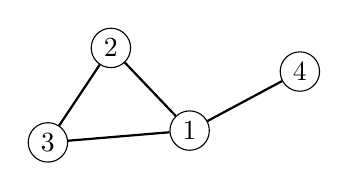
\begin{tikzpicture}[x=2.0cm,y=1.5cm]
            \tikzset{     
            e4c node/.style={circle,draw,minimum size=0.5cm,inner sep=0}, 
            e4c edge/.style={sloped,above,font=\footnotesize}
            }
            \node[e4c node] (1) at (0.9, 0.1) {1}; 
            \node[e4c node] (2) at (0.4, 0.8) {2}; 
            \node[e4c node] (3) at (0.0, 0.0) {3}; 
            \node[e4c node] (4) at (1.6, 0.6) {4}; 
            
            \path[-,draw,thick]
            (1) edge[e4c edge] (2)
            (1) edge[e4c edge] (3)
            (1) edge[e4c edge] (4)
            (2) edge[e4c edge] (3)
            ;
        \end{tikzpicture}
    \end{wrapfigure}
    W zbiorze wierzchołków grafu na rysunku obok istnieją dwa dwuelementowe niezależne podzbiory: $\{2, 4\}$ oraz $\{3, 4\}$.
    \bigskip

    Skojarzeniem $E_G$ jest na przykład $\big\{\{2, 3\}, \{1, 4\}\big\}$ i to skojarzenie jest doskonałe.
\end{example}

\textbf{Drzewo} to graf spójny bez cykli. Następujące warunki są równoważne:
\begin{enumerate}
    \item $G$ jest drzewem.
    \item Każde dwa wierzchołki w $G$ są połączone dokładnie jedną drogą.
    \item $G$ jest minimalny spójny.
    \item $G$ jest maksymalny acykliczny.
    \item $G$ jest spójny i $|V| = |E| + 1$.
\end{enumerate}

\subsection{Cykle Eulera i Hamiltona}
\textbf{Cykl Eulera} w grafie to cykl przechodzący przez każdą krawędź dokładnie raz. Powiemy, że graf jest \textbf{eulerowski}, gdy zawiera cykl Eulera.

Warunek konieczny i wystarczający: graf spójny $G$ jest eulerowski wtedy i tylko wtedy, gdy \purple{każdy jego wierzchołek jest parzystego stopnia}, a dla grafów skierowanych -- każdy wierzchołek ma równy stopień wyjściowy i wejściowy.
\bigskip

\textbf{Cykl Hamiltona} to cykl przechodzący przez każdy wierzchołek dokładnie raz. Powiemy, że graf jest \textbf{hamiltonowski}, gdy zawiera cykl Hamiltona.

W przeciwieństwie do cyklu Eulera, ogólny problem rozstrzygnięcia, czy dany graf ma cykl Hamiltona, jest zwykle bardzo trudny.

\begin{example}
    \begin{wrapfigure}{r}{8.3cm}
        \vspace{4mm}
        
        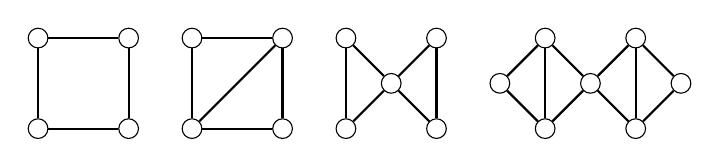
\begin{tikzpicture}[x=1.15cm,y=1.15cm]
            \tikzset{     
            e4c node/.style={circle,draw,minimum size=0.25cm,inner sep=0}, 
            e4c edge/.style={sloped,above,font=\footnotesize}
            }
            \node[e4c node] (1) at (0.0, 1.0) {}; 
            \node[e4c node] (2) at (0.0, 0.0) {}; 
            \node[e4c node] (3) at (1.0, 0.0) {}; 
            \node[e4c node] (4) at (1.0, 1.0) {}; 
            \node[e4c node] (1a) at (1.7, 1.0) {}; 
            \node[e4c node] (2a) at (1.7, 0.0) {}; 
            \node[e4c node] (3a) at (2.7, 0.0) {}; 
            \node[e4c node] (4a) at (2.7, 1.0) {};
            \node[e4c node] (1b) at (3.4, 1.0) {}; 
            \node[e4c node] (2b) at (3.4, 0.0) {}; 
            \node[e4c node] (3b) at (3.9, 0.5) {}; 
            \node[e4c node] (4b) at (4.4, 0.0) {};
            \node[e4c node] (5b) at (4.4, 1.0) {};
            \node[e4c node] (1c) at (5.1, 0.5) {}; 
            \node[e4c node] (2c) at (5.6, 1.0) {}; 
            \node[e4c node] (3c) at (5.6, 0.0) {}; 
            \node[e4c node] (4c) at (6.1, 0.5) {}; 
            \node[e4c node] (5c) at (6.6, 0.0) {};
            \node[e4c node] (6c) at (6.6, 1.0) {};
            \node[e4c node] (7c) at (7.1, 0.5) {}; 
            
            \path[-,draw,thick]
            (4) edge[e4c edge] (3)
            (3) edge[e4c edge] (2)
            (2) edge[e4c edge] (1)
            (1) edge[e4c edge] (4)
            (4a) edge[e4c edge] (3a)
            (3a) edge[e4c edge] (2a)
            (2a) edge[e4c edge] (1a)
            (1a) edge[e4c edge] (4a)
            (2a) edge[e4c edge] (4a)
            (1b) edge[e4c edge] (2b)
            (1b) edge[e4c edge] (3b)
            (2b) edge[e4c edge] (3b)
            (3b) edge[e4c edge] (4b)
            (3b) edge[e4c edge] (5b)
            (4b) edge[e4c edge] (5b)
            (1c) edge[e4c edge] (2c)
            (1c) edge[e4c edge] (3c)
            (2c) edge[e4c edge] (3c)
            (2c) edge[e4c edge] (4c)
            (3c) edge[e4c edge] (4c)
            (4c) edge[e4c edge] (5c)
            (4c) edge[e4c edge] (6c)
            (5c) edge[e4c edge] (6c)
            (5c) edge[e4c edge] (7c)
            (6c) edge[e4c edge] (7c)
            ;
        \end{tikzpicture}
    \end{wrapfigure}
    Na rysunku znajdują się kolejno przykłady grafu:
    \begin{itemize}
        \item eulerowskiego i hamiltonowskiego
        \item nieeulerowskiego, ale hamiltonowskiego
        \item eulerowskiego, ale niehamiltonowskiego
        \item nieeulerowskiego i niehamiltonowskiego
    \end{itemize}
\end{example}

\subsection{Grafy dwudzielne}

Graf $G$ jest grafem \textbf{dwudzielnym}, jeśli $V_G = V_1 \cup V_2$, gdzie $V_1$ i $V_2$ są rozłącznymi zbiorami wierzchołków i~każda krawędź ma jeden koniec w~$V_1$, a drugi w~$V_2$.

\textbf{Graf pełny dwudzielny} $K_{n, m}$ to taki, w którym $|V_1| = n, |V_2| = m$ oraz każdy wierzchołek z $V_1$ jest połączony z każdym innym z $V_2$.

Warunek konieczny i wystarczający: graf jest dwudzielny wtedy i tylko wtedy, gdy \purple{nie zawiera cykli nieparzystej długości}.
\bigskip

Skojarzenia (zbiory niezależnych krawędzi) w grafach dwudzielnych to \textbf{Systemy Różnych Reprezentantów} (SRR). Koncept ten jest wykorzystywany przy rozwiązywaniu niektórych problemów z teorii zbiorów, jak na poniższym przykładzie.

\begin{example}
    \begin{wrapfigure}{r}{5cm}
        \vspace{-4mm}
    
        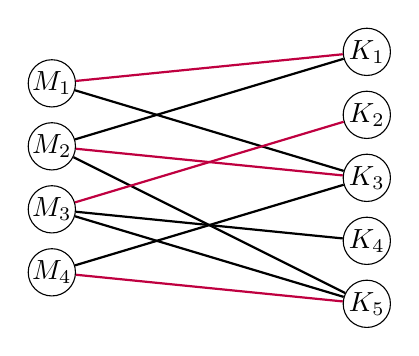
\begin{tikzpicture}[x=2cm,y=2cm]
            \tikzset{     
            e4c node/.style={circle,draw,minimum size=0.6cm,inner sep=0}, 
            e4c edge/.style={sloped,above,font=\footnotesize}
            }
            \node[e4c node] (M1) at (0.0, 1.4) {$M_1$}; 
            \node[e4c node] (M2) at (0.0, 1.0) {$M_2$}; 
            \node[e4c node] (M3) at (0.0, 0.6) {$M_3$}; 
            \node[e4c node] (M4) at (0.0, 0.2) {$M_4$}; 
            \node[e4c node] (K1) at (2.0, 1.6) {$K_1$}; 
            \node[e4c node] (K2) at (2.0, 1.2) {$K_2$}; 
            \node[e4c node] (K3) at (2.0, 0.8) {$K_3$}; 
            \node[e4c node] (K4) at (2.0, 0.4) {$K_4$}; 
            \node[e4c node] (K5) at (2.0, 0.0) {$K_5$}; 
            
            \path[-,draw,thick]
            (M1) edge[e4c edge, purple] (K1)
            (M1) edge[e4c edge] (K3)
            (M2) edge[e4c edge] (K1)
            (M2) edge[e4c edge, purple] (K3)
            (M2) edge[e4c edge] (K5)
            (M3) edge[e4c edge, purple] (K2)
            (M3) edge[e4c edge] (K4)
            (M3) edge[e4c edge] (K5)
            (M4) edge[e4c edge] (K3)
            (M4) edge[e4c edge, purple] (K5)
            ;
        \end{tikzpicture}
    \end{wrapfigure}

    Chcemy wybrać żony dla mężczyzn $M_1, ..., M_4$ wśród kandydatek $K_1, ..., K_5$, tak aby każdy mężczyzna ożenił się z kobietą, którą zna. 
    \bigskip
    
    Sporządźmy (dwudzielny) graf znajomości: jeśli $M_i$ zna $K_j$, to odpowiednie wierzchołki połączymy krawędzią.
    \bigskip

    Rozwiązaniem problemu jest wybór Systemu Różnych Reprezentantów, na przykład odpowiadającego skojarzeniu $$\big\{\{M_1, K_1\}, \{M_2, K_3\}, \{M_3, K_2\}, \{M_4, K_5\}\big\}$$
\end{example}

Naturalnie nasuwającym się pytaniem jest to, kiedy System Różnych Reprezentantów dla danego grafu dwudzielnego w ogóle istnieje. Odpowiedź przynosi nam \textbf{twierdzenie Halla}. Okazuje się, że warunkiem koniecznym i wystarczającym na istnienie SRR jest to, by \purple{każda podgrupa $k$ kobiet znała co najmniej $k$ mężczyzn}.

\subsection{Planarność}

\textbf{Płaskie włożenie} grafu w płaszczyznę to przedstawienie go graficznie w postaci, w której jego krawędzie nie przecinają się. Graf, który ma takie włożenie, nazywamy \textbf{planarnym}.

\textbf{Ścianą} w płaskim włożeniu nazywać będziemy maksymalny spójny obszar płaszczyzny rozłączny z grafem. Jedna ze ścian (zewnętrzna) jest nieograniczona.

\begin{example}
    Poniżej przedstawiono klikę $K_4$ i jej płaską reprezentację, wraz z wyróżnionymi ścianami. Płaskie włożenie uzyskano, przesuwając wierzchołek z lewego górnego rogu zgodnie ze strzałką.
    \begin{center}
        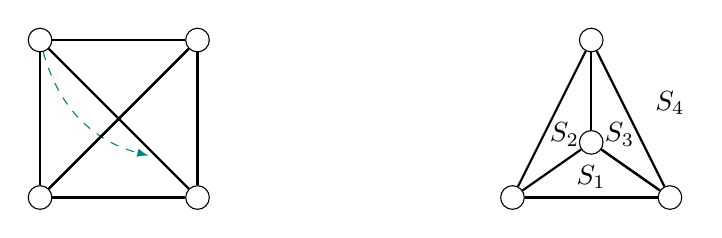
\begin{tikzpicture}[x=2cm,y=2cm]
            \tikzset{     
            e4c node/.style={circle,draw,minimum size=0.3cm,inner sep=0}, 
            e4c edge/.style={sloped,above,font=\footnotesize}
            }
            \node[e4c node] (1) at (0.0, 1.0) {}; 
            \node[e4c node] (2) at (0.0, 0.0) {}; 
            \node[e4c node] (3) at (1.0, 0.0) {}; 
            \node[e4c node] (4) at (1.0, 1.0) {}; 
            \node[e4c node] (1a) at (3.0, 0.0) {}; 
            \node[e4c node] (2a) at (4.0, 0.0) {}; 
            \node[e4c node] (3a) at (3.5, 1.0) {}; 
            \node[e4c node] (4a) at (3.5, 0.35) {};
            \node[] (M) at (0.75, 0.25) {};
            \node[] (S1) at (3.5, 0.13) {$S_1$};
            \node[] (S2) at (3.33, 0.4) {$S_2$};
            \node[] (S3) at (3.68, 0.4) {$S_3$};
            \node[] (S4) at (4.0, 0.6) {$S_4$};

            \path[-latex, bend right = 30, teal, dashed]
            (1) edge[] (M);
            
            \path[-,draw,thick]
            (1) edge[e4c edge] (2)
            (2) edge[e4c edge] (3)
            (3) edge[e4c edge] (4)
            (4) edge[e4c edge] (1)
            (1) edge[e4c edge] (3)
            (2) edge[e4c edge] (4)
            (2) edge[e4c edge] (4)
            (1a) edge[e4c edge] (2a)
            (2a) edge[e4c edge] (3a)
            (3a) edge[e4c edge] (4a)
            (4a) edge[e4c edge] (1a)
            (1a) edge[e4c edge] (3a)
            (2a) edge[e4c edge] (4a)
            (2a) edge[e4c edge] (4a)
            ;
        \end{tikzpicture}
    \end{center}
\end{example}

Liczba ścian płaskiego włożenia grafu spełnia \textbf{wzór Eulera}:
$$\purple{v - e + f = 2,}$$
gdzie $v$ -- liczba wierzchołków, $e$ -- liczba krawędzi, $f$ -- liczba ścian. Ze wzoru Eulera otrzymujemy górne oszacowanie liczby krawędzi w grafie planarnym:
$$\text{dla } v \geq 3 \text{ zachodzi } \purple{e \leq 3v - 6},$$
z którego wynika, że na przykład graf $K_5$ jest nieplanarny.

Dla grafów niezawierających trójkątów (cykli długości 3) prawdziwa jest jeszcze mocniejsza teza:
$$\purple{e \leq 2v - 4},$$
z której wiadomo, że graf dwudzielny $K_{3, 3}$ także jest nieplanarny. Z powyższych wzorów można też wywnioskować, że \purple{każdy graf planarny zawiera wierzchołek stopnia $\leq 5$}, co stanowi warunek konieczny planarności.
\bigskip

Grafy $G$ i $H$ nazwiemy \textbf{homeomorficznymi}, jeśli można je uczynić izomorficznymi poprzez dostawianie wierzchołków na ich krawędziach. Dla przykładu, poniższe dwa grafy są homeomorficzne.
\begin{center}
    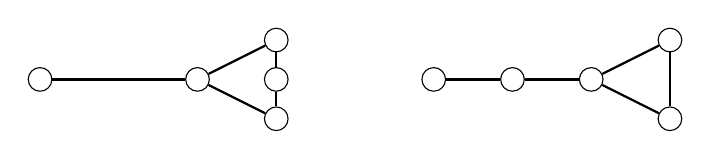
\begin{tikzpicture}[x=1cm,y=1cm]
        \tikzset{     
        e4c node/.style={circle,draw,minimum size=0.3cm,inner sep=0}, 
        e4c edge/.style={sloped,above,font=\footnotesize}
        }
        \node[e4c node] (1) at (0.0, 0.5) {}; 
        \node[e4c node] (2) at (2.0, 0.5) {}; 
        \node[e4c node] (3) at (3.0, 1.0) {}; 
        \node[e4c node] (4) at (3.0, 0.5) {}; 
        \node[e4c node] (5) at (3.0, 0.0) {}; 
        \node[e4c node] (1a) at (5.0, 0.5) {}; 
        \node[e4c node] (2a) at (6.0, 0.5) {}; 
        \node[e4c node] (3a) at (7.0, 0.5) {}; 
        \node[e4c node] (4a) at (8.0, 1.0) {}; 
        \node[e4c node] (5a) at (8.0, 0.0) {}; 
        
        \path[-,draw,thick]
        (1) edge[e4c edge] (2)
        (2) edge[e4c edge] (3)
        (3) edge[e4c edge] (4)
        (4) edge[e4c edge] (5)
        (5) edge[e4c edge] (2)
        (1a) edge[e4c edge] (2a)
        (2a) edge[e4c edge] (3a)
        (3a) edge[e4c edge] (4a)
        (4a) edge[e4c edge] (5a)
        (5a) edge[e4c edge] (3a)
        ;
    \end{tikzpicture}
\end{center}

Warunek konieczny i wystarczający istnienia płaskiego włożenia grafu opisuje \textbf{twierdzenie Kuratowskiego}: graf jest nieplanarny wtedy i tylko wtedy, gdy \purple{zawiera podgraf homeomorficzny z $K_5$ lub $K_{3,3}$}.

\begin{exam}
    Dany jest graf $G$ o $n \leq 6$ wierzchołkach i $m$ krawędziach. Wówczas
    \answers{$G$ lub dopełnienie $G$ jest planarne}{jeśli $m < 10$, to $G$ jest planarny}{jeśli $m > 10$, to $G$ nie jest planarny}
    \bigskip

    Rozwiążemy podpunkt \textbf{A.} Dla $n \leq 4$ jasne jest, że $G$ jest planarny (twierdzenie Kuratowskiego). Dla $n = 5$ jedynym istniejącym grafem nieplanarnym $G$ jest $K_5$, ale wtedy dopełnienie $G$ jest planarne. Rozpatrzmy $n = 6$ i załóżmy, że $G$ jest nieplanarny. Z twierdzenia Kuratowskiego wynika, że $G$ zawiera podgraf homeomorficzny z $K_5$ lub $K_{3, 3}$.
    
    Podgraf homeomorficzny z $K_5$ ma 5 wierzchołków stopnia 4. Jeśli podgrafem homeomorficznym w $G$ jest $K_5$, to dopełnienie $G$ ma przynajmniej 5 wierzchołków stopnia $< 2$, więc na podstawie twierdzenia Kuratowskiego dopełnienie $G$ jest planarne.

    Z drugiej strony, jeśli $G$ zawierałoby podgraf homeomorficzny z $K_{3,3}$, to skoro $G$ ma 6 wierzchołków, musi być $G = K_{3,3}$ i wtedy dopełnienie $G$ jest planarne. Podpunkt \textbf{A.} jest więc prawdziwy.
    \bigskip

    Do pozostałych podpunktów nietrudno znaleźć kontrprzykłady: dla podpunktu \textbf{B.} wystarczy wziąć $G = K_{3,3}$, a dla podpunktu \textbf{C.} graf z rysunku poniżej ($n = 6, m = 11$). Oba te stwierdzenia są więc fałszywe.
    
    \begin{center}
    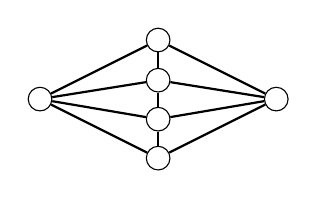
\begin{tikzpicture}[x=1.5cm,y=1.5cm]
        \tikzset{     
        e4c node/.style={circle,draw,minimum size=0.3cm,inner sep=0}, 
        e4c edge/.style={sloped,above,font=\footnotesize}
        }
        \node[e4c node] (1) at (0.0, 0.5) {}; 
        \node[e4c node] (2) at (1.0, 1.0) {}; 
        \node[e4c node] (3) at (1.0, 0.66) {}; 
        \node[e4c node] (4) at (1.0, 0.33) {}; 
        \node[e4c node] (5) at (1.0, 0.0) {};
        \node[e4c node] (6) at (2.0, 0.5) {};
        
        \path[-,draw,thick]
        (1) edge[e4c edge] (2)
        (1) edge[e4c edge] (3)
        (1) edge[e4c edge] (4)
        (1) edge[e4c edge] (5)
        (2) edge[e4c edge] (3)
        (3) edge[e4c edge] (4)
        (4) edge[e4c edge] (5)
        (6) edge[e4c edge] (2)
        (6) edge[e4c edge] (3)
        (6) edge[e4c edge] (4)
        (6) edge[e4c edge] (5)
        ;
    \end{tikzpicture}
    \end{center}
\end{exam}

\subsection{Kolorowanie grafów}

\textbf{Kolorowanie grafu} $G$ za pomocą $k$ kolorów to funkcja $f : V_G \to \{1, ..., k\}$ przyporządkowująca kolory wierzchołkom w taki sposób, że każde dwa wierzchołki połączone krawędzią są w różnych barwach.

Najmniejsze $k$, dla którego istnieje $k$-kolorowanie $G$, nazywamy \textbf{liczbą chromatyczną} $\chi(G)$. Znalezienie jej jest w ogólnym przypadku trudne. 
\bigskip

Istnieje szereg twierdzeń pomagających znaleźć liczbę chromatyczną. Jednym z nich jest \textbf{twierdzenie o czterech barwach}:
$$\purple{\text{jeśli graf jest planarny, to } \chi(G) \leq 4}.$$

Ponadto, z prostej obserwacji wynika, że
$$\purple{\chi(G) = 2 \wtw G \text{ jest dwudzielny}}.$$

Łącząc powyższe informacje, otrzymujemy wniosek, że graf planarny niebędący grafem dwudzielnym jest zawsze albo 3-, albo 4-kolorowalny. Okazuje się jednak, że sprawdzenie tej informacji dla danego grafu jest problemem NP-trudnym.
\bigskip

\begin{wrapfigure}{r}{2cm}
    \vspace{-5mm}
    
    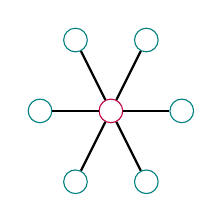
\begin{tikzpicture}[x=1.8cm,y=1.8cm]
        \tikzset{     
        e4c node/.style={circle,draw,minimum size=0.3cm,inner sep=0}, 
        e4c edge/.style={sloped,above,font=\footnotesize}
        }
        \node[e4c node, purple] (S) at (0.5, 0.5) {};
        \node[e4c node, teal] (1) at (0.25, 1.0) {}; 
        \node[e4c node, teal] (2) at (0.75, 1.0) {}; 
        \node[e4c node, teal] (3) at (1.0, 0.5) {}; 
        \node[e4c node, teal] (4) at (0.75, 0.0) {};
        \node[e4c node, teal] (5) at (0.25, 0.0) {};
        \node[e4c node, teal] (6) at (0.0, 0.5) {};
        
        \path[-,draw,thick]
        (S) edge[e4c edge] (1)
        (S) edge[e4c edge] (2)
        (S) edge[e4c edge] (3)
        (S) edge[e4c edge] (4)
        (S) edge[e4c edge] (5)
        (S) edge[e4c edge] (6)
        ;
    \end{tikzpicture}
\end{wrapfigure}

Innym narzędziem pozwalającym ograniczyć liczbę chromatyczną z góry jest \textbf{twierdzenie Brooksa}. Oznaczmy jako $\Delta(G)$ maksymalny stopień wierzchołka w grafie $G$. Jeśli spójny graf $G$ nie jest cyklem nieparzystej długości ani kliką, to $\purple{\chi(G) \leq \Delta(G)}$.

Ale uwaga: to oszacowanie może być bardzo niedokładne, na przykład gwiazda (rysunek obok) ma $\chi(G) = 2$ i dowolnie duże $\Delta(G)$ (wystarczy dokładać wierzchołki na brzegu i łączyć je z środkowym).
\bigskip

Wyróżniamy także \textbf{kolorowanie krawędziowe}, czyli funkcję $f : E_G \to \{1, ..., k\}$, taką że incydentne krawędzie są różnego koloru. Analogicznie, \textbf{indeks chromatyczny} $\chi_e(G)$ to najmniejsze $k$, dla którego istnieje $k$-kolorowanie krawędziowe.

Po krótkim rozumowaniu łatwo znaleźć dolne oszacowanie indeksu chromatycznego: $\chi_e(G) \geq \Delta(G)$, jednakże o dodatkowym, nieoczywistym fakcie mówi \textbf{twierdzenie Vizinga}: $$\chi_e(G) \leq \Delta(G) + 1.$$

W związku z tym \purple{indeks chromatyczny $\chi_e(G)$ jest zawsze równy albo $\Delta(G)$, albo $\Delta(G) + 1$} (dla dowolnego $G$). Mimo to rozstrzygnięcie, który wariant jest prawdziwy dla danego grafu, jest w ogólnym przypadku trudne. Jeśli jednak graf $G$ jest dwudzielny, to $\chi_e(G) = \Delta(G)$.

\begin{problems}
    \prob Graf $G$ ma cykl Eulera, ale nie ma cyklu Hamiltona. Wynika z tego, że
    \answers{dopełnienie grafu $G$ ma cykl Hamiltona}{$G$ ma ścieżkę Hamiltona}{$G$ ma więcej niż jedną dwuspójną składową}

    \prob Każdy graf nieplanarny o $n$ wierzchołkach
    \answers{zawiera podgraf $K_{3,3}$ lub $K_5$}{ma co najmniej $3n-5$ krawędzi}{ma liczbę chromatyczną nie mniejszą niż 5}

    \prob Graf $100$-wierzchołkowy $G$ ma liczbę chromatyczną $3$. Wynika z tego, że graf $G$
    \answers{jest planarny}{zawiera cykl}{zawiera niezależny zbiór wierzchołków rozmiaru $34$}

    \prob Dany jest $k$-regularny graf o $n$ wierzchołkach i $m$ krawędziach. Wtedy
    \answers
    {$k$ jest parzyste lub $n$ jest parzyste}
    {$k$ jest dzielnikiem $n$}
    {$k$ jest dzielnikiem $m$}

    \prob $G$ jest grafem spójnym o $n > 2$ wierzchołkach i takim, że każda jego krawędź należy do pewnego cyklu prostego. Wynika z tego, że
    \answers
    {$G$ ma cykl Hamiltona}
    {graf otrzymany przez usunięcie z $G$ jednego wierzchołka jest spójny}
    {każde dwa różne wierzchołki w $G$ są połączone przynajmniej dwiema krawędziowo rozłącznymi ścieżkami}

    \prob Graf $G$ ma $n > 2$ wierzchołków i $n$ krawędzi. Wynika z tego, że graf $G$
    \answers
    {jest spójny}
    {zawiera cykl}
    {jest planarny}

    \prob $G$ jest $n$-wierzchołkowym grafem spójnym regularnym stopnia 3. Wynika z tego, że
    \answers{$n$ jest parzyste}{$G$ jest planarny}{liczba chromatyczna $\chi(G) \leq 4$}
\end{problems}

% Grześ
\section{Teoria liczb}

Na wstępie, przypomnijmy sobie podstawowe definicje i notacje związane z podzielnością liczb.
\begin{itemize}
    \item Dla $b>0$ i dowolnego $a$ istnieją jednoznacznie wyznaczone $q$ (\textbf{iloraz}) i $0\leq r<b$ (\textbf{reszta}) takie, że $a=b\cdot q + r$.

    \item \textbf{Największy wspólny dzielnik} (NWD) liczb $a,b$ to liczba $s$ taka, że $s\mid a,b$ oraz jeśli $d\mid a,b$, to także $d\mid s$. $\mathrm{NWD}(a,b)$ to najmniejszy dodatni element zbioru $\{ax+by : x,y\in\ZZ\}$.
    
    \item Jeśli $\mathrm{NWD}(a,b)$ jest równe 1, to $a$ i $b$ są \textbf{względnie pierwsze} ($a\perp b$).

    \item Znane jest \textbf{podstawowe twierdzenie arytmetyki}: każda liczba $a>0$ ma rozkład $a=\prod_{i=1}^{n}p_i$, gdzie $p_i$ to \textbf{czynniki pierwsze}, który jest jednoznaczny z dokładnością do kolejności elementów.
\end{itemize}







\begin{example}
    Niech $a=p_1^{\alpha_1}p_2^{\alpha_2}\cdots p_k^{\alpha_k}$ oraz $b=p_1^{\beta_1}p_2^{\beta_2}\cdots p_k^{\beta_k}$, gdzie $p_i$ to różne czynniki pierwsze. Wtedy
    \begin{itemize}
        \item $b\mid a \wtw \forall_i \ \beta_i\leq\alpha_i$
        \item $b\perp a \wtw \forall_i \ \min(\alpha_i,\beta_i)=0$
        \item $\mathrm{NWD}(a,b)=\prod_{i=1}^k p_i^{\min(\alpha_i,\beta_i)}$
        \item $\purple{\mathrm{NWW}(a,b)=\frac{ab}{\mathrm{NWD}(a,b)}}=\prod_{i=1}^k p_i^{\max(\alpha_i,\beta_i)}$
    \end{itemize}
\end{example}

\begin{exam}
    Dla dowolnych dodatnich liczb całkowitych $a$ i $b$ zachodzi implikacja
    \answers{$a^2 \ | \ b^2 \Rightarrow a^3 \ | \ b^3$}{$a^2 \ | \ b^3 \Rightarrow a \ | \  b$}{$a^3 \ | \  b^2 \Rightarrow a \ | \  b$}
    \begin{enumerate}[\bf A.]
        \item Skoro $a^2$ dzieli $b^2$, to możemy zapisać, że $b^2=ka^2$ dla pewnego $k\in\ZZ$. Stąd $k=\frac{b^2}{a^2}=(\frac{b}{a})^2$. Widzimy, że $a$ musi być dzielnikiem $b$, ponieważ $k$ ma być całkowite. Skoro $a\mid b$, to również $a^3\mid b^3$, więc odpowiedź to \texttt{TAK}.
        \item Weźmy $a=2^3$ i~$b=2^2$. Oczywiście $a^2=2^6=b^3$, więc $a^2\mid b^3$, ale $a\nmid b$, więc odpowiedź to \texttt{NIE}.
        \item Podobnie jak w podpunkcie \textbf{A.}, zapiszmy daną relację jako $b^2=ka^3$ dla pewnego $k\in\ZZ$. Stąd $ak=(\frac{b}{a})^2$. Skoro $ak$ jest liczbą całkowitą (jako iloczyn liczb całkowitych), to $\frac{b}{a}$ również musi być całkowite, więc $a\mid b$ i odpowiedzią jest \texttt{TAK}.
    \end{enumerate}
\end{exam}

\subsection{Algorytm Euklidesa}

Algorytm Euklidesa pozwala efektywnie wyznaczyć $\mathrm{NWD}(a,b)$ oraz $x,y$ takie, że $\mathrm{NWD}(a,b)=ax+by$:
\begin{itemize}
    \item jeśli $b=0$, to $\langle x,y\rangle\leftarrow\langle1,0\rangle$
    \item wpp. mamy $x',y'$ takie, że $\mathrm{NWD}(a,b)=\mathrm{NWD}(b,a\mod{b})=bx'+(a\mod{b})y'$, ale $a\mod{b}=a-b\cdot\left\lfloor\frac{a}{b}\right\rfloor$, więc można przyjąć $\langle x,y\rangle\leftarrow\langle y',x'-y'\cdot\left\lfloor\frac{a}{b}\right\rfloor\rangle$
\end{itemize}

\begin{example}
    Znajdziemy $x,y$, dla których $\mathrm{NWD}(36,15)=36x+15y$:
    $$
    \begin{matrix}
        a & b & & x & y \\
        36 & 15 & \downarrow\ \uparrow & \purple{-2} & \purple{5} \\
        15 & 6 & \downarrow\ \uparrow & 1 & -2 \\
        6 & 3 & \downarrow\ \uparrow & 0 & 1 \\
        3 & 0 & \rightarrow & 1 & 0
    \end{matrix}
    $$
    Na początku stosujemy wzór $\mathrm{NWD}(a,b)=\mathrm{NWD}(b,a\mod{b})$ tak długo, dopóki nie otrzymamy 0 w drugiej kolumnie. Następnie korzystamy z pierwszego przypadku i przypisujemy wartości $\langle x,y\rangle\leftarrow\langle1,0\rangle$. Idąc do góry, stosujemy wzór $\langle x,y\rangle\leftarrow\langle y',x'-y'\cdot\left\lfloor\frac{a}{b}\right\rfloor\rangle$. Ostatecznie otrzymujemy
    $$\mathrm{NWD}(36,15)=36\cdot\purple{(-2)}+15\cdot\purple{5}=3$$
\end{example}

\subsection{Kongruencje}

Dla $n>0$ mówimy, że \textbf{$a$ przystaje do $b$ modulo $n$} ($a\equiv b\mod{n}$), gdy $n\mid a-b$, czyli $a$ i $b$ dają tę samą resztę z dzielenia przez $n$.

Własności kongruencji:
\begin{itemize}
    \item $\equiv$ (mod $n$) jest relacją równoważności, jako zbiór reprezentantów jej klas abstrakcji można wziąć $Z_n=\{0,\ldots,n-1\}$
    \item kongruencje można dodawać, odejmować, mnożyć i potęgować stronami (jak równania)
    \item kongruencję $a\equiv b$ (mod $n$) można podzielić obustronnie przez $d$ tylko, gdy $d\perp n$
    \item $ad\equiv bd\mod{nd}\wtw a\equiv b\mod{n}$
\end{itemize}
\bigskip

Jeśli $n_1\perp n_2$, to układ dwóch kongruencji
$$
\begin{cases}
    a \equiv b \mod{n_1} \\
    a \equiv b \mod{n_2}
\end{cases}
$$
jest równoważny pojedynczej kongruencji $a\equiv b\mod{n_1n_2}$. Na tym prostym spostrzeżeniu bazuje dużo silniejsze \textbf{chińskie twierdzenie o resztach}:

Niech $n=n_1\cdots n_k$, gdzie $n_i$ parami względnie pierwsze. Wtedy dla dowolnych $a_1,\ldots,a_k$ istnieje dokładnie jedno $a\in\{0,\ldots,n-1\}$ takie, że
$$a \equiv a_i \mod{n_i}, \text{ dla } i\in\{1,\ldots,k\}$$

\begin{example}
    Niech $\langle n_1,n_2,n_3\rangle = \langle7,11,13\rangle$ i wtedy $n=1001$. Weźmy $\langle a_1,a_2,a_3\rangle = \langle5,3,11\rangle$ i znajdźmy $a$ takie, że $a$ daje resztę $a_i \mod{n_i}$ dla $i=1,2,3$.

    Znajdujemy $m_i$ takie, że $n_j\mid m_i$ dla $j\neq i$ oraz $m_i\perp n_i$ (na przykład $m_i=\frac{n}{n_i}$) i przyjmujemy
    $$a=\sum_i(a_im_i(m_i^{-1}\mod{n_i}))\mod{n},$$
    gdzie $m^{-1}\mod{n}$ to odwrotność modularna, czyli takie $x$, że $mx\equiv1\mod{n}$. Odwrotność modularną łatwo znaleźć za pomocą algorytmu Euklidesa jako współczynnik przy $m_i$ w wyrażeniu $m_ix+n_iy=\mathrm{NWD}(m_i,n_i)=1$. U nas
    $$a=(5\cdot143\cdot5+3\cdot91\cdot4+11\cdot77\cdot12)\mod{1001}=817$$
\end{example}

Inne, często wykorzystywane przy kongruencjach twierdzenie to \textbf{małe twierdzenie Fermata}: jeśli $p$ jest liczbą pierwszą i $p\nmid a$, to $\purple{a^{p-1}\equiv1\mod{p}}$.

\subsection{Funkcja Eulera}

Niech $Z_n^*=\{1\leq k\leq n : k\perp n\}$, czyli zbiór liczb całkowitych dodatnich niewiększych niż $n$ i względnie pierwszych z $n$. \textbf{Funkcja Eulera} $\Phi:\NN\to\NN$ jest określona jako $\Phi(n)=|Z_n^*|$, czyli liczba liczb mniejszych od $n$ względnie pierwszych z $n$.

Własności:
\begin{itemize}
    \item jeśli $p$ jest pierwsza, to $\Phi(p^k)=p^k-p^{k-1}$
    \item multiplikatywność: jeśli $m\perp n$, to $\Phi(mn)=\Phi(m)\Phi(n)$
    \item wzór iloczynowy: $\Phi(n)=n\prod_{p\mid n}(1-\frac{1}{p})$, gdzie $p$ jest pierwsza
\end{itemize}

Funkcja Eulera pozwala nam uogólnić małe twierdzenie Fermata -- w ten sposób powstało \textbf{twierdzenie Eulera}: jeśli $a\perp n$, to $\purple{a^{\Phi(n)}\equiv1\mod{n}}$.

\begin{example}
    Obliczymy $2^{65536}$ mod 2009 za pomocą twierdzenia Eulera. Mamy $2009 = 7^2\cdot41$, więc korzystając z własności funkcji Eulera:
    $$\Phi(2009)=\Phi(7^2)\Phi(41)=42\cdot40=1680$$
    Stąd dostajemy
    $$2^{1680}\equiv1\mod{2009}$$
    Znajdziemy teraz iloraz i resztę z dzielenia 65536 przez 1680:
    $$65536=1680\cdot q+r=1680\cdot39+16$$
    To pozwoli nam dojść do szukanego wyrażenia -- podnosimy kongruencję stronami do potęgi $q=39$, a następnie przemnażamy stronami przez $2^r=2^{16}$:
    $$2^{1680\cdot39+16}\equiv2^{16}\mod{2009}$$
    stąd
    $$2^{65536}\equiv65536\equiv1248\mod{2009}$$
    Trzeba jednak pamiętać, że twierdzenia Eulera możemy używać jedynie, gdy $a\perp n$. W naszym przypadku $n=7^2\cdot41$, więc oczywiście jest względnie pierwsze z $a=2$.
\end{example}

\begin{problems}
    \prob Liczba $p > 2$ jest pierwsza. Wynika z tego, że
    \answers{$(p-2)^{p-1}-1$ dzieli się przez $p$}{$(p-2)^{p^2-1}-1$ dzieli się przez $p^2$}{$(p-2)^{p^3-p^2}-1$ dzieli się przez $p^3$}

    \prob Jeśli $a, b$ są dodatnimi liczbami całkowitymi, to $\mathrm{NWD}(a,b)$ jest najmniejszym dodatnim elementem zbioru
    \answers{$\{ax + by \mid x, y \in \mathbb{Z}\}$}{$\{a(x+y) + b(x-y) \mid x, y \in \mathbb{Z}\}$}{$\{2ax + 3by \mid x,y \in \mathbb{Z}\}$}

    \prob Dane są dodatnie liczby całkowite $a, b$, których największy wspólny dzielnik jest równy $d$. Wówczas względnie pierwsze są liczby
    \answers{$\frac{a}{d}$ oraz $b$}{$\frac{ab}{d^2}$ oraz $b$}{$\frac{a^2}{d^2}$ oraz $\frac{b^2}{d^2}$}
\end{problems}

% Błażej
\section{Asymptotyka}

\textbf{Notacja asymptotyczna} pozwala ukryć zbędne nadmiarowe informacje, uprościć operowanie wyrażeniami i~ocenić przybliżone graniczne zachowanie.

Jeśli $f, g : \NN \to \RR^+$, to zapisujemy $\purple{f = O(g)}$, gdy dla pewnej stałej $c$ i dostatecznie dużych $n$ zachodzi
$$f(n) \leq c \cdot g(n)$$

Zapis $f = O(g)$ czytamy jako ,,$f$ \textbf{jest co najwyżej rzędu} $g$'' albo ,,$f$ rośnie co najwyżej tak szybko, jak $g$''.

Inne stosowane oznaczenia:
\begin{itemize}
    \item $\purple{f = \Omega(g)} \wtw g = O(f)$ \hfill ,,$f$ rośnie co najmniej tak szybko, jak $g$"
    \item $\purple{f = \Theta(g)} \wtw f = O(g) \land g = O(f)$ \hfill ,,$f$ rośnie tak samo szybko, jak $g$"
    \item $\purple{f = o(g)} \wtw \Limn \frac{f(n)}{g(n)} = 0$ \hfill ,,$f$ rośnie istotnie wolniej niż $g$"
    \item $\purple{f = \omega(g)} \wtw g = o(f) \wtw \Limn \frac{f(n)}{g(n)} = \infty$ \hfill ,,$f$ rośnie istotnie szybciej niż $g$"
    \item $\purple{f \sim g} \wtw \Limn \frac{f(n)}{g(n)} = 1$ \hfill ,,$f$ jest asymptotycznie równe $g$"
\end{itemize}

Definicja notacji asymptotycznej jest ściśle powiązana z definicją granicy. Istotnie, jeśli wartość $\Limn \frac{f(n)}{g(n)}$ jest określona, możemy z niej wywnioskować relację asymptotyczną między $f$ i $g$:
$$\Limn \frac{f(n)}{g(n)} \neq \infty \ \Rightarrow \ f = O(g), \qquad \Limn \frac{f(n)}{g(n)} \neq 0 \ \Rightarrow \ f = \Omega(g),$$
$$\Limn \frac{f(n)}{g(n)} \neq 0, \infty \ \Rightarrow \ f = \Theta(g)$$

Powszechnie znane są także zależności asymptotyczne między charakterystycznymi funkcjami. Oznaczmy $f < g$, jeśli $f = o(g)$. Wtedy dla dowolnych $a \in (0, 1)$ i $b > 1$ zachodzi:
$$\purple{\frac{1}{b^n} < \frac{1}{n^b} < 1 < (\log \log n)^b < \log n < n^a < n < n \log n < n^b < b^n < n!}$$

\subsection{Twierdzenie o rekurencji uniwersalnej}

Równania rekurencyjne typu ,,\textbf{dziel i zwyciężaj}'' są postaci
$$\purple{T(n) = a \cdot T\left(\floor{\frac{n}{b}}\right) + f(n)},$$
gdzie $f$ jest funkcją nieujemną oraz $a, b \in \RR^+$. Tak zdefiniowana funkcja $T$ stanowi pewien schemat działania algorytmów typu ,,dziel i zwyciężaj'' -- problem o rozmiarze $n$ dzielony jest na $a$ podproblemów, każdy wielkości $\floor{\frac{n}{b}}$, funkcja $f$ przedstawia koszt dzielenia problemu oraz połączenia rozwiązań podproblemów.

W ogólnej postaci powyższego równania można \textbf{zignorować podłogi i sufity} (łatwo pokazać, że asymptotycznie nie zmieni to rozwiązania).

Takie równania łatwo rozwiązujemy, korzystając z \textbf{twierdzenia o rekurencji uniwersalnej}:
\begin{itemize}
    \item jeśli $f(n) = O(n^{\log_b a - \epsilon})$ dla pewnej stałej $\epsilon > 0$, to $\purple{T(n) = \Theta(n^{\log_b a})}$
    \item jeśli $f(n) = \Theta(n^{\log_b a})$, to $\purple{T(n) = \Theta(n^{\log_b a} \log n)}$
    \item jeśli $f(n) = \Omega(n^{\log_b a + \epsilon})$ dla pewnej stałej $\epsilon > 0$ i jeżeli $a \cdot f(\frac{n}{b}) \leq c \cdot f(n)$ dla pewnej stałej $c \in (0, 1)$ i~dostatecznie dużych $n$, to $\purple{T(n) = \Theta(f(n))}$
\end{itemize}

Intuicyjnie, każdy z trzech przypadków rekurencji uniwersalnej sprowadza się do stwierdzenia, która z funkcji $n^{\log_b a}$ i $f$ jest ,,większa''. Gdy znana jest odpowiedź na to pytanie, automatycznie znane jest asymptotyczne ograniczenie danej rekursji -- jest nią owa ,,większa'' funkcja.

\begin{example}
    Koszt rozwiązania algorytmu wyszukiwania binarnego opisuje równanie
    $$T(n) = T\left(\frac{n}{2}\right) + O(1).$$
    Korzystając z twierdzenia o rekurencji uniwersalnej, odczytujemy $a = 1, b = 2$ i wtedy $f(n) = \Theta(n^{\log_2 1}) = \Theta(1)$. Stąd otrzymujemy rozwiązanie $T(n) = O(\log n)$.
\end{example}

\begin{problems}
    \prob Funkcje $f, g: \NN \rightarrow \RR$ przyjmują wyłącznie wartości dodatnie i są niemalejące. Wynika z tego, że
    \answers{jeśli $f = O(g)$ i $g = O(f)$, to istnieje skończona granica $\Limn \frac{f(n)}{g(n)}$}{jeśli $f = O(g)$, to $f/g = O(1)$}{$f = O(g)$ lub $g = O(f)$}

    \prob Rozwiązaniem równania rekurencyjnego $T(n)=2T(\lfloor n/2 \rfloor)+f(n)$ dla $n>1$, $T(1)=0$, jest
    \answers{$T(n)=\Theta(\log{n})$, jeśli $f(n)=O(1)$}{$T(n)=\Theta(n)$, jeśli $f(n)=\Theta(\sqrt{n})$}{$T(n)=\Theta(n^2)$, jeśli $f(n)=\Theta(n^2)$}
\end{problems}

\begin{solutions}
    % Jasiek
    \sol Niech $f$ oznacza permutację $\lr{3, 6, 1, 4, 2, 5}$ i niech $f^k$ oznacza $k$-krotne złożenie permutacji $f$. Wynika z tego, że
    \answerss{$f^8 = \lr{1, 2, 3, 4, 5, 6}$}{$f^7=f$}{$f^4=f^{16}$}{NIE}{TAK}{TAK}

    Rozważmy zapis cyklowy danej permutacji: $[1, 3][2, 6, 5][4]$. Rozmiary tych cykli to kolejno 2, 3, 1. To oznacza, że $f^6 = id$, gdzie $id$ to permutacja identycznościowa. Z tego powodu dla dowolnego $k$ mamy $f^k = f^{k + 6}$ i po odpowiednim podstawieniu łatwo uzyskujemy odpowiedzi do zadania.

    % Kasia
    \sol Jeśli ponumerujemy permutacje zbioru $\{1, 2, 3, 4, 5\}$ od $1$ do $120$ w porządku leksykograficznym, to permutacją o numerze $60$ będzie
    \answerss
    {$\lr{3, 5, 1, 2, 4}$}
    {$\lr{3, 4, 1, 2, 5}$}
    {$\lr{3, 2, 5, 4, 1}$}
    {NIE}{NIE}{TAK}
    Jak łatwo zauważyć, permutacji z określoną liczbą na pierwszym miejscu jest dokładnie $4!=24$. Możemy zatem określić, że permutacje z numerami 1-24 mają jako pierwszą liczbę ,,1'', numery 25-48 -- liczbę ,,2'', a numery 49-72 -- liczbę ,,3''. Wiemy również, że permutacji z określonymi liczbami na pierwszych dwóch miejscach jest dokładnie $3!=6$. Zatem możemy określić, że permutacje z numerami 49-54 mają jako początek $\lr{3, 1}$, a numery 55-60 -- początek $\lr{3, 2}$. Stąd wniosek, że sześćdziesiątą permutacją będzie największa w porządku leksykograficznym permutacja o początku $\lr{3, 2}$ i jest nią permutacja $\lr{3, 2, 5, 4, 1}$. 

    % Kasia
    \sol Liczba permutacji liczb (1, ..., 2021) takich, że ,,1'' jest w cyklu parzystej długości, jest równa
    \answerss{$2021!/2$}{$1010 \cdot 2020!$}{$1011 \cdot 2020!$}{NIE}{TAK}{NIE}

    Szukane permutacje w postaci superzapisu mają liczbę ,,1'' na $(2k+1)$-szym miejscu od końca dla $0 \leq k \leq 1009$. Tworząc takie zapisy, najpierw na $2020!$ sposobów układamy liczby (2, ..., 2021), a następnie na jeden z $1010$ sposobów wybieramy, gdzie znajdzie się liczba ,,1''. Takich permutacji jest więc dokładnie $1010 \cdot 2020!$, stąd tylko odpowiedź \textbf{B.} jest poprawna.

    % Tomek
    \sol Niech $A(x)$ będzie funkcją tworzącą ciągu $\lr{a_n}_{n \in \NN}$.
    \answerss{$\frac{A(x)}{1 - x}$ jest funkcją tworzącą ciągu $\lr{a_0 + a_1 + ... + a_n}_{n \in \NN}$}{$A^2(x)$ jest funkcją tworzącą ciągu $\lr{a_n^2}_{n \in \NN}$}{$xA(x)$ jest funkcją tworzącą ciągu $\lr{a_{n+1}}_{n \in \NN}$}{TAK}{NIE}{NIE}
    \begin{enumerate}[\bf A.]
        \item Splot dowolnego ciągu z ciągiem samych jedynek tworzy ciąg sum częściowych (łatwo to pokazać, korzystając wprost z definicji splotu). Odpowiedź jest więc prawdziwa.
        \item Tożsamość nie jest prawdziwa, z definicji splotu otrzymujemy
        $$A(x)A(x) \leftrightarrow \lr{\sum_k a_k a_{n - k}}_{n \in \NN}$$
        a to nie musi być $\lr{a_n^2}_{n \in \NN}$.
        \item Nie, ponieważ $xA(x) \leftrightarrow \lr{0, a_0, a_1, \ldots}$ -- to przesunięcie w prawo, a nie w lewo.
    \end{enumerate}

    % Błażej
    \sol Funkcją tworzącą $A(x)$ ciągu $\lr{(n+1)2^n}_{n \in \NN}$ jest
    \answerss{$\frac{1}{(1-2x)(1-x)}$}{$\frac{\text{d}}{\dx}\frac{1}{1-2x}$}{$\int_0^x\frac{\dt}{1-2t}$}{NIE}{NIE}{NIE}

    \begin{enumerate}[\bf A.]
        \item Zauważmy, że wyrażenie można rozpisać jako iloczyn dwóch szeregów geometrycznych:
        $$\frac{1}{1 - 2x} \cdot \frac{1}{1 - x} = (1 + 2x + 4x^2 + 8x^3 + ...)(1 + x + x^2 + x^3 + ...),$$
        a to jest splot funkcji tworzących ciągów $\lr{1, 2, 4, 8, ...} = \lr{2^n}_{n \in \NN}$ oraz $\lr{1, 1, 1, ...}$. Jak wiemy, splot dowolnego ciągu z ciągiem samych jedynek tworzy ciąg sum częściowych. Stąd $$\frac{1}{(1 - 2x)(1 - x)} \leftrightarrow \lr{\sum_{k = 0}^n 2^k}_{n \in \NN}$$
        i odpowiedź to \texttt{NIE}.

        \item Z definicji różniczkowania funkcji tworzącej:
        $$\left(\frac{1}{1 - 2x}\right)' = (1 + 2x + 4x^2 + 8x^3 + ...)' = 2 + 8x + 24x^2 + ... \leftrightarrow \lr{(n + 1)2^{n + 1}}_{n \in \NN}$$
        Odpowiedź jest więc fałszywa.

        \item Z definicji całkowania funkcji tworzącej:
        $$\int_0^x\frac{\dt}{1-2t} = \int_0^x (1 + 2t + 4t^2 + 8t^3 + ...) \dt = x + \frac{2}{2} x^2 + \frac{4}{3} x^3 + \frac{8}{4} x^4 + ... \leftrightarrow \lr{\frac{2^{n - 1}}{n}}_{n \in \NN}$$
        Odpowiedź jest więc fałszywa.
    \end{enumerate}

    % Julia
    \sol Niech $A(x)$ będzie funkcją tworzącą (zwykłą) ciągu $\lr{a_n}_{n \in \NN}$. Wynika z tego, że funkcją tworzącą ciągu
    \answerss
    {$\lr{-a_n}_{n \in \NN}$ jest $A(-x)$}
    {$\lr{2^n a_n}_{n \in \NN}$ jest $A(2x)$}
    {$\lr{\sum_{k=0}^n a_k}_{n \in \NN}$ jest $\frac{A(x)}{1-x}$}
    {NIE}{TAK}{TAK}

    Odpowiedzi w podpunktach \textbf{A.} i \textbf{B.} wynikają z własności podstawienia do funkcji tworzących. W podpunkcie \textbf{A.} mamy $$A(-x) \leftrightarrow \lr{(-1)^n a_n}_{n \in \NN} \neq \lr{-a_n}_{n \in \NN}$$ Podpunkt \textbf{B.} także jest spełniony na podstawie wspomnianej własności.
    
    Prawdziwość podpunktu \textbf{C.} wynika z faktu, że splot
    dowolnego ciągu z ciągiem samych jedynek tworzy ciąg sum częściowych (a funkcja $\frac{1}{1-x} = 1 + x + x^2 + ...$ to funkcja tworząca ciągu samych jedynek).

    % Michał
    \sol Liczba sposobów na umieszczenie $n > 0$ nierozróżnialnych kul w $k > 0$ rozróżnialnych komorach to współczynnik przy wyrazie
    \answerss{$x^n$ funkcji $(1-x)^{-k}$}{$x^k$ funkcji $(1-x)^{-n}$}{$x^{k-1}$ funkcji $(1-x)^{-n-1}$}{TAK}{NIE}{TAK}

    Problem z zadania jest analogiczny do problemu wybierania $n$-kombinacji z powtórzeniami z $k$-elementowego zbioru. Enumeratorem jest więc $$(1 + x + x^2 + \dots)^k = \left(\frac{1}{1 - x}\right)^k = (1 - x)^{-k},$$zatem przy podpunkcie \textbf{A.} odpowiedzią jest \texttt{TAK}.

    Za pomocą metody \textit{stars and bars} możemy również sprawdzić, że szukana w zadaniu liczba sposobów jest równa $\binom{n + k - 1}{n}$. 
    
    Enumerator z podpunktu \textbf{B.} odpowiada umieszczaniu $N = k$ nierozróżnialnych kul w $K = n$ rozróżnialnych komorach, zatem liczba sposobów to $\binom{N + K - 1}{N} = \binom{n + k - 1}{k} \neq \binom{n + k - 1}{n}$, 
    odpowiedź to \texttt{NIE}.

    Enumerator z podpunktu \textbf{C.} odpowiada umieszczaniu $N = k - 1$ nierozróżnialnych kul w $K = n + 1$ nierozróżnialnych komorach, zatem liczba sposobów to $\binom{N + K - 1}{N} = \binom{n + k - 1}{k - 1} = \binom{n + k - 1}{n}$ i odpowiedź jest prawdziwa.

    % Patryk
    \sol Dany jest ciąg $a_n = |\{\langle A, x \rangle: A \subseteq \{1, ..., n\}, x \in A\}|$. Wtedy
    \answerss{$\Limn \frac{a_{n + 1}}{a_n} = \infty$}{$a_n$ jest parzyste dla $n \geq 2$}{$a_n = n \cdot n!$ dla $n > 0$}{NIE}{TAK}{NIE}
    Obliczymy kolejne wyrazy ciągu $(a_n)_{n \in \NN}$. Chcemy dowiedzieć się, ile jest par składających się ze zbioru i liczby zawartej w tym zbiorze. Liczbę $x$ możemy wybrać na $n$ sposobów. Natomiast liczba zbiorów zawierających $x$ to $2^{n-1}$ (połowa wszystkich możliwych zbiorów, ponieważ $x$ w 50\% przypadków należy do zbioru, a w 50\% nie należy).
    
    Mamy więc $a_n = 2^{n-1} \cdot n$, co rozwiązuje podpunkt \textbf{C.} W podpunkcie \textbf{A.} możemy łatwo zauważyć, że granica wynosi 2, a w podpunkcie \textbf{B.}, że faktycznie dla $n \geq 2$ wyrazy ciągu są parzyste.

    % Patryk
    \sol Liczba podzbiorów zbioru 2018-elementowego o mocy co najwyżej 1009 jest równa
    \answerss
    {liczbie podzbiorów zbioru 2018-elementowego o mocy większej niż 1009}
    {$\binom{2018}{1009}$}
    {$2^{2017}$}
    {NIE}{NIE}{NIE}
    
    Obliczymy wymaganą liczbę podzbiorów. Zauważmy symetrię wynikającą z dwumianu Newtona: $$\binom{2018}{0} = \binom{2018}{2018}, \quad \binom{2018}{1} = \binom{2018}{2017}, \quad ...$$ Możemy zauważyć, że $\binom{2018}{1008} = \binom{2018}{1010}$, natomiast $\binom{2018}{1009}$ jest bez pary, więc \textbf{A.} jest fałszywe.
    
    Podpunkt \textbf{B.} to liczba podzbiorów o mocy równej 1009, a nie \textit{co najwyżej} 1009 -- odpowiedź jest fałszywa.
    
    Przy podpunkcie \textbf{C.} możemy zauważyć, że $2^{2017}$ to połowa mocy zbioru potęgowego o 2018 elementach, a -- jak pokazaliśmy wyżej przy podpunkcie \textbf{A.} -- liczba podzbiorów o mocy co najwyżej 1009 jest większa niż połowa, więc odpowiedź jest fałszywa.

    \sol Liczba par $(A, B)$, takich że $A, B \subseteq \{1, 2, ..., 2023\}$ oraz
    \answerss{$A \subseteq B$ jest równa $3^{2023}$}{$A \cap B = \pusty$ jest równa $3^{2023}$}{$|A \cup B|$ jest liczbą parzystą, jest równa $3^{2023}$}
    {TAK}{TAK}{NIE}

    \begin{enumerate}[\bf A.]
        \item Każdy element zbioru $\{1, 2, ..., 2023\}$ może
        \begin{itemize}
            \item należeć jednocześnie do $A$ i $B$,
            \item należeć wyłącznie do $B$,
            \item nie należeć ani do $A$, ani do $B$.
        \end{itemize}
        Nietrudno sprawdzić, że takie przyporządkowanie elementów pozwoli nam jednoznacznie zliczyć odpowiednie pary $(A, B)$. Odpowiedź jest więc prawdziwa -- dla każdego z 2023 elementów mamy do podjęcia jeden z trzech wyborów.

        \item Rozumowanie analogiczne jak przy podpunkcie \textbf{A.}: każdy element zbioru $\{1, 2, ..., 2023\}$ może
        \begin{itemize}
            \item należeć do $A$ (ale nie do $B$),
            \item należeć do $B$ (ale nie do $A$),
            \item nie należeć ani do $A$, ani do $B$.
        \end{itemize}
        Odpowiedź jest prawdziwa.

        \item Tym razem każdy element zbioru $\{1, 2, ..., 2023\}$ może
        \begin{itemize}
            \item należeć jednocześnie do $A$ i $B$,
            \item należeć do $A$ (ale nie do $B$),
            \item należeć do $B$ (ale nie do $A$),
            \item nie należeć ani do $A$, ani do $B$.
        \end{itemize}

        Interesują nas jednak tylko te przypadki, w których $|A \cup B|$ jest parzyste, lub równoważnie: liczba elementów nienależących ani do $A$, ani do $B$ jest nieparzysta. Nietrudno sprawdzić, że to dokładnie połowa wszystkich możliwych przypadków (tutaj pominiemy to rozumowanie). Szukaną więc liczbą par $(A, B)$ w podpunkcie \textbf{C.} jest $4^{2023}/2 \neq 3^{2023}$.
    \end{enumerate}

    % Grześ
    \sol Graf $G$ ma cykl Eulera, ale nie ma cyklu Hamiltona. Wynika z tego, że
    \answerss{dopełnienie grafu $G$ ma cykl Hamiltona}{$G$ ma ścieżkę Hamiltona}{$G$ ma więcej niż jedną dwuspójną składową}{NIE}{NIE}{NIE}
    
    Rozważmy następujące grafy spełniające warunki zadania:

    \begin{center}
    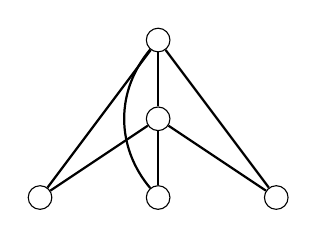
\begin{tikzpicture}[x=4cm, y=2cm, scale = 0.25]
        \tikzset{     
        e4c node/.style={circle,draw,minimum size=0.3cm,inner sep=0}, 
        e4c edge/.style={sloped,above,font=\footnotesize}
        }
        \node[e4c node] (1) at (0, 0) {};
        \node[e4c node] (2) at (0, -2) {};
        \node[e4c node] (3) at (-1.5, -4) {};
        \node[e4c node] (4) at (0, -4) {};
        \node[e4c node] (5) at (1.5, -4) {};

        \path[-,draw,thick]
        (1) edge[e4c edge] (2)
        (1) edge[e4c edge] (3)
        (1) edge[e4c edge] (5)
        (2) edge[e4c edge] (3)
        (2) edge[e4c edge] (4)
        (2) edge[e4c edge] (5)
        (4) edge[e4c edge, bend left = 40] (1)
        ;
    \end{tikzpicture}
    \qquad
    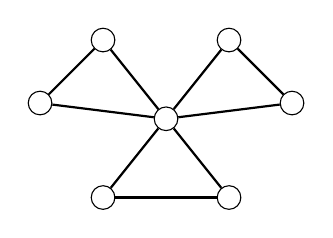
\begin{tikzpicture}[x=4cm,y=2cm]
        \tikzset{     
        e4c node/.style={circle,draw,minimum size=0.3cm,inner sep=0}, 
        e4c edge/.style={sloped,above,font=\footnotesize}
        }
        \node[e4c node] (1) at (3.6, 0.6) {}; 
        \node[e4c node] (2) at (3.8, 1.0) {}; 
        \node[e4c node] (3) at (3.8, 0.0) {}; 
        \node[e4c node] (4) at (4.0, 0.5) {};
        \node[e4c node] (5) at (4.2, 0.0) {};
        \node[e4c node] (6) at (4.2, 1.0) {};
        \node[e4c node] (7) at (4.4, 0.6) {};
        
        \path[-,draw,thick]
        (1) edge[e4c edge] (2)
        (1) edge[e4c edge] (4)
        (2) edge[e4c edge] (4)
        (3) edge[e4c edge] (4)
        (3) edge[e4c edge] (5)
        (4) edge[e4c edge] (5)
        (4) edge[e4c edge] (6)
        (4) edge[e4c edge] (7)
        (6) edge[e4c edge] (7)
        ;
    \end{tikzpicture}
    \end{center}

    \begin{enumerate}[\bf A.]
        \item W dopełnieniach obydwu grafów ich środkowy wierzchołek będzie odizolowany, więc nie może istnieć tam cykl Hamiltona.

        \item Graf po prawej nie ma ścieżki Hamiltona.

        \item Graf po lewej jest dwuspójny, więc posiada tylko jedną dwuspójną składową -- samego siebie.
    \end{enumerate}

    % Wiktor
    \sol Każdy graf nieplanarny o $n$ wierzchołkach
    \answerss{zawiera podgraf $K_{3,3}$ lub $K_5$}{ma co najmniej $3n-5$ krawędzi}{ma liczbę chromatyczną nie mniejszą niż 5}{NIE}{NIE}{NIE}
    \begin{enumerate}[\bf A.]
        \item Graf nieplanarny jest z $K_5$ lub $K_{3,3}$ homeomorficzny, ale nie oznacza to, że któryś z nich jest jego podgrafem.
        \item Kontrprzykładem jest $K_{3, 3}$ (9 krawędzi, 6 wierzchołków).
        \item Wiemy, że jeśli graf jest planarny, to jego liczba chromatyczna jest mniejsza bądź równa 4, ale nie jest to implikacja obustronna. Graf $K_{3,3}$ ma liczbę chromatyczną $2$.
    \end{enumerate}

    % Patryk
    \sol Graf $100$-wierzchołkowy $G$ ma liczbę chromatyczną $3$. Wynika z tego, że graf $G$
    \answerss{jest planarny}{zawiera cykl}{zawiera niezależny zbiór wierzchołków rozmiaru $34$}{NIE}{TAK}{TAK}

    Możemy o takim grafie pomyśleć jak o grafie \textit{trójdzielnym} -- dzielimy 100 wierzchołków na 3 zbiory, każdy odpowiadający jednemu kolorowi. Krawędź może wystąpić tylko między wierzchołkami o różnych kolorach (wynika to wprost z definicji kolorowania grafu).

    \begin{enumerate}[\bf A.]
        \item Weźmy oszacowanie na liczbę krawędzi w grafie planarnym: $e \leq 3v-6$. Wynika z niego, że w grafie $G$ mogą być co najwyżej 294 krawędzie. Weźmy graf, w którym są 33 wierzchołki niebieskie, 33 zielone i 34 czerwone. Połączmy ze sobą wszystkie niebieskie i zielone wierzchołki, otrzymując $33^2 = 1089 > 294$ krawędzi, więc taki graf nie jest planarny.

        \item Gdyby graf $G$ nie zawierał cyklu, jego liczba chromatyczna byłaby równa 2 (moglibyśmy pokolorować wierzchołki dwoma kolorami, na przemian) -- sprzeczność z założeniem.

        \item Przy podzieleniu 100 wierzchołków na 3 zbiory, jeden z nich będzie miał moc co najmniej 34 (zasada szufladkowa), więc można znaleźć w nim podzbiór 34 niezależnych wierzchołków.
    \end{enumerate}
    
    % Julia
    \sol Dany jest $k$-regularny graf o $n$ wierzchołkach i $m$ krawędziach. Wtedy
    \answerss
    {$k$ jest parzyste lub $n$ jest parzyste}
    {$k$ jest dzielnikiem $n$}
    {$k$ jest dzielnikiem $m$}
    {TAK}{NIE}{NIE}

    \begin{enumerate}[\bf A.]
        \item Z definicji $k$-regularnego grafu wiemy, że z każdego wierzchołka wychodzi $k$ krawędzi. Z lematu o uściskach dłoni otrzymujemy równanie $kn = 2m$. Ponieważ $m$ jest liczbą naturalną, $k$ lub $n$ musi być parzyste.
        \item Kontrprzykładem jest $K_5$.
        \item Kontrprzykładem jest $K_3$.
    \end{enumerate}

    % Grześ
    \sol $G$ jest grafem spójnym o $n > 2$ wierzchołkach i takim, że każda jego krawędź należy do pewnego cyklu prostego. Wynika z tego, że
    \answerss
    {$G$ ma cykl Hamiltona}
    {graf otrzymany przez usunięcie z $G$ jednego wierzchołka jest spójny}
    {każde dwa różne wierzchołki w $G$ są połączone przynajmniej dwiema krawędziowo rozłącznymi ścieżkami}
    {NIE}{NIE}{TAK}
    Rozważmy następujący graf spełniający warunki zadania:
    \begin{center}
        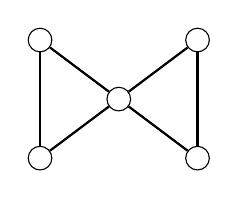
\begin{tikzpicture}[x=2cm,y=1.5cm]
            \tikzset{     
            e4c node/.style={circle,draw,minimum size=0.3cm,inner sep=0}, 
            e4c edge/.style={sloped,above,font=\footnotesize}
            }
            \node[e4c node] (1) at (3.4, 1.0) {}; 
            \node[e4c node] (2) at (3.4, 0.0) {}; 
            \node[e4c node] (3) at (3.9, 0.5) {}; 
            \node[e4c node] (4) at (4.4, 0.0) {};
            \node[e4c node] (5) at (4.4, 1.0) {};
            
            \path[-,draw,thick]
            (1) edge[e4c edge] (2)
            (1) edge[e4c edge] (3)
            (2) edge[e4c edge] (3)
            (3) edge[e4c edge] (4)
            (3) edge[e4c edge] (5)
            (4) edge[e4c edge] (5)
            ;
        \end{tikzpicture}
    \end{center}
    
    Nietrudno sprawdzić, że nie ma on cyklu Hamiltona, a po usunięciu środkowego wierzchołka graf się rozspójni. Wobec tego odpowiedzi \textbf{A.} i \textbf{B.} są fałszywe. 
    
    Zauważmy, że w grafie $G$ danym w treści zadania nie mogą wystąpić mosty (krawędzie rozspójniające) -- gdyby w grafie był most, krawędź ta musiałaby należeć do cyklu prostego, co jest niemożliwe, gdyż po przejściu przez most nie jesteśmy już w stanie ,,wrócić'', żeby zamknąć cykl. Skoro nie ma mostów, to usunięcie dowolnej krawędzi z grafu go nie rozspójnia.
    
    Weźmy więc ścieżkę pomiędzy dowolnymi dwoma wierzchołkami $u$ i $v$. Usuwając wszystkie krawędzie na ścieżce, graf wciąż jest spójny, więc istnieje druga, rozłączna krawędziowo z pierwszą, ścieżka z $u$ do $v$. Stąd odpowiedź w \textbf{C.} to \texttt{TAK}.

    % Wiktor
    \sol Graf $G$ ma $n > 2$ wierzchołków i $n$ krawędzi. Wynika z tego, że graf $G$
    \answerss
    {jest spójny}
    {zawiera cykl}
    {jest planarny}
    {NIE}{TAK}{NIE}
    
    \begin{enumerate}[\bf A.]
        \item Nie musi tak być -- weźmy $K_4$ (4 wierzchołki, 6 krawędzi) i dorzućmy dwa izolowane wierzchołki.
        \item Gdyby $G$ nie zawierał żadnego cyklu, to byłby drzewem. Jak wiemy, drzewa to spójne grafy spełniające zależność $|V| = |E| + 1$, więc w naszym przypadku, chcąc dołożyć $n$-tą krawędź, utworzylibyśmy cykl.
        \item Kontrprzykład: bierzemy $K_5$ i dokładamy tyle izolowanych wierzchołków, żeby ich liczba była równa liczbie krawędzi.
    \end{enumerate}

    \sol $G$ jest $n$-wierzchołkowym grafem spójnym regularnym stopnia 3. Wynika z tego, że
    \answerss{$n$ jest parzyste}{$G$ jest planarny}{liczba chromatyczna $\chi(G) \leq 4$}
    {TAK}{NIE}{TAK}

    \begin{enumerate}[\bf A.]
        \item Oznaczmy przez $m$ liczbę krawędzi grafu z zadania. Z lematu o uściskach dłoni otrzymujemy zależność $3n = 2m$ i -- ponieważ $n$ i $m$ to liczby naturalne -- nietrudno zauważyć, że $n$ musi być parzyste.
        
        \item Kontrprzykładem jest $K_{3, 3}$.

        \item Ponieważ każdy wierzchołek grafu $G$ jest połączony z dokładnie trzema innymi, mamy pewność, że wystarczą nam 4 barwy do prawidłowego pokolorowania grafu. 
    \end{enumerate}

    % Grześ
    \sol Liczba $p > 2$ jest pierwsza. Wynika z tego, że
    \answerss{$(p-2)^{p-1}-1$ dzieli się przez $p$}{$(p-2)^{p^2-1}-1$ dzieli się przez $p^2$}{$(p-2)^{p^3-p^2}-1$ dzieli się przez $p^3$}{TAK}{NIE}{TAK}
    Nietrudno zauważyć, że $(p-2)\perp p$. Możemy więc skorzystać z małego twierdzenia Fermata, otrzymując ${(p-2)^{p-1}\equiv 1\mod{p}}$. Zatem podpunkt \textbf{A.} jest prawdziwy.
    
    Skoro $(p-2)\perp p$, to również $(p-2)\perp p^3$ oraz $\Phi(p^3)=p^3-p^2$, bo $p$ jest pierwsze. Z twierdzenia Eulera dostajemy $(p-2)^{p^3-p^2}\equiv 1\mod{p^3}$, więc podpunkt \textbf{C.} również jest prawdziwy.
    
    Do podpunktu \textbf{B.} posłuży nam kontrprzykład: weźmy najmniejszą (sensowną) liczbę pierwszą $p=5$. Obliczamy:
    \begin{align*}
        (p-2)^{p^2-1} &\mod p^2 \\
        (5-2)^{25-1} &\mod 25 \\
        3^{24} &\mod 25
    \end{align*}
    Widzimy, że $3^3\equiv 27\equiv 2\mod{25}$. Podnosimy tę kongruencję stronami do potęgi 8 i dostajemy $3^{24}\equiv 2^8\equiv 256\equiv 6\nequiv 1\mod{25}$. Odpowiedź jest więc fałszywa.

    % Jasiek
    \sol Jeśli $a, b$ są dodatnimi liczbami całkowitymi, to $\mathrm{NWD}(a,b)$ jest najmniejszym dodatnim elementem zbioru
    \answerss{$\{ax + by \mid x, y \in \mathbb{Z}\}$}{$\{a(x+y) + b(x-y) \mid x, y \in \mathbb{Z}\}$}{$\{2ax + 3by \mid x,y \in \mathbb{Z}\}$}{TAK}{NIE}{NIE}
    Prawdziwa odpowiedź do podpunktu \textbf{A.} wynika wprost z definicji NWD. W podpunkcie \textbf{B.} rozważmy $a = 9, b = 15$ (wtedy NWD$(a, b) = 3$). Dla pewnych $x, y$ musi zachodzić:
    \begin{align*}
        9(x + y) + 15(x - y) = 3 \wtw 3(x + y) + 5(x - y) = 1 \wtw 8x - 2y = 1
    \end{align*}
    To prowadzi do sprzeczności, ponieważ po lewej stronie równości znajduje się liczba nieparzysta, a~po prawej parzysta.
    
    W podpunkcie \textbf{C.} przeprowadzamy taką samą argumentację dla $a = 2, b = 4$ i~ponownie uzyskujemy sprzeczność: $$4x + 12y = 2 \wtw 2x + 6y = 1$$
    
    % Grześ
    \sol Dane są dodatnie liczby całkowite $a, b$, których największy wspólny dzielnik jest równy $d$. Wówczas względnie pierwsze są liczby
    \answerss{$\frac{a}{d}$ oraz $b$}{$\frac{ab}{d^2}$ oraz $b$}{$\frac{a^2}{d^2}$ oraz $\frac{b^2}{d^2}$}{NIE}{NIE}{TAK}
    
    Połóżmy $a=d\cdot a'$ i $b=d\cdot b'$, gdzie $d$ to $\mathrm{NWD}(a,b)$. Oczywiście $a'\perp b'$. Podpunkt \textbf{A.} jest fałszywy, bo o ile $a'\perp b'$, to nieprawdą jest, że $a'\perp d$; nie musi tak być chociażby dla $a=2^2$ i $b=2\cdot3$. Ten przykład pokazuje również, że \textbf{B.} nie ma sensu (z tego samego powodu).
    
    Podpunkt \textbf{C.} jest jednak prawdziwy, gdyż $\frac{a^2}{d^2}=(a')^2$, $\frac{b^2}{d^2}=(b')^2$, a skoro $a'\perp b'$, to oczywiście $(a')^2\perp (b')^2$.

    % Patryk
    \sol Funkcje $f, g: \NN \rightarrow \RR$ przyjmują wyłącznie wartości dodatnie i są niemalejące. Wynika z tego, że
    \answerss{jeśli $f = O(g)$ i $g = O(f)$, to istnieje skończona granica $\Limn \frac{f(n)}{g(n)}$}{jeśli $f = O(g)$, to $f/g = O(1)$}{$f = O(g)$ lub $g = O(f)$}{NIE}{TAK}{NIE}

    \begin{enumerate}[\bf A.]
        \item Taka granica nie musi istnieć. Kontrprzykładem mogą być funkcje
        $$f(n) = n, \qquad g(n) = \begin{cases}
            n & \text{dla } n \text{ nieparzystych,} \\
            2n & \text{dla } n \text{ parzystych.}
        \end{cases}$$
        
        \item Z definicji notacji asymptotycznej mamy, że dla pewnej stałej $c$ i dostatecznie dużych $n$ zachodzi $$f(n) \leq c \cdot g(n), \quad \text{ a stąd } \quad \frac{f(n)}{g(n)} \leq c.$$ 

        \item Rozważmy funkcje
        $$
        f(n) = 
        \begin{cases}
            (n - 1)^2 & \text{dla } n \text{ nieparzystych,} \\
            n^2 & \text{dla } n \text{ parzystych,}
        \end{cases}
        $$
    
        $$
        g(n) = 
        \begin{cases}
            n^2 & \text{dla } n \text{ nieparzystych,} \\
            (n - 1)^2 & \text{dla } n \text{ parzystych,}
        \end{cases}
        $$
        będące ciągami kwadratowymi, przy czym raz rośnie $f$, a raz $g$. Wówczas różnica $|f(n)-g(n)|$ wraz ze wzrostem $n$ dąży do nieskończoności oraz $\big(f(n)-g(n)\big)\big(f(n+1)-g(n+1)\big) < 0$.
    \end{enumerate}

    % Grześ
    \sol Rozwiązaniem równania rekurencyjnego $T(n)=2T(\lfloor n/2 \rfloor)+f(n)$ dla $n>1$, $T(1)=0$, jest
    \answerss{$T(n)=\Theta(\log{n})$, jeśli $f(n)=O(1)$}{$T(n)=\Theta(n)$, jeśli $f(n)=\Theta(\sqrt{n})$}{$T(n)=\Theta(n^2)$, jeśli $f(n)=\Theta(n^2)$}{NIE}{TAK}{TAK}
    
    Korzystamy z twierdzenia o rekurencji uniwersalnej. Odczytujemy $a=b=2$, więc nasze $f(n)$ musimy dopasować do jednego z trzech przypadków:
    \begin{enumerate}[1.]
        \item $f(n)=O(n^{\log_b{a}-\epsilon})=O(n^{1-\epsilon})$,
        \item $f(n)=\Theta(n^{\log_b{a}})=\Theta(n)$,
        \item $f(n)=\Omega(n^{\log_b{a}+\epsilon})=\Omega(n^{1+\epsilon})$.
    \end{enumerate}

    \begin{enumerate}[\bf A.]
        \item Skoro $f(n)=O(1)$, to otrzymujemy pierwszy przypadek. Rozwiązaniem równania rekurencyjnego będzie $T(n)=\Theta(n^{\log_ba})=\Theta(n)$, czyli odpowiedź to \texttt{NIE}.

        \item Skoro $f(n)=\Theta(\sqrt{n})$, to znów jesteśmy w przypadku pierwszym i rozwiązaniem jest $T(n)=\Theta(n)$, czyli odpowiedź to \texttt{TAK}.

        \item Jeśli $f(n)=\Theta(n^2)$, to wpadamy do trzeciego przypadku, więc rozwiązaniem jest $T(n)=\Theta(f(n))=\Theta(n^2)$, czyli \texttt{TAK}.
    \end{enumerate}
\end{solutions}